\chapter{Limited Geometry}
\label{chap:analSimulations}

\section{Electromagnetic modes excitation}
\label{sec:anal_DAW_modeExcitation}

As an introduction to simulations with SOLEDGE3X, let us consider the linear behavior of drift-Alfvén waves again. To put later simulation results in perspective, we analyze the impact of electromagnetic terms on drift-wave turbulence within a linearized system. Specifically, we compare the effects of a finite electron mass (EI-inert), electromagnetic induction with electron mass (EM), and electromagnetic induction with both flutter and electron mass (EM-flutter) in comparison to the baseline electrostatic case. The dispersion relation from Eq. \ref{eq:edge_DAWdispersionRelation} is adjusted to each of the four scenarios and solved exactly using the Python library SymPy for symbolic computation. Notably, we use the full dispersion relation without applying the simplifications used when we introduced the linear behavior of the drift-Alfvén system in Sec. \ref{ssec:edge_DAW_dispersionRelation}. To recall, the dispersion relation is given by: 

´\begin{equation}
	\label{eq:anal_DAWdispersionRelation}
	i\left(\rho_{L,e}^2k_\perp^2 + \beta_0\right)\omega^3 + \left(-i\beta_0\omega_* - \frac{\eta_\parallel en_0T_0k_\perp^2}{B^2}\right)\omega^2 - i\omega_s^2\left(\omega_*-\left(1 + \rho_L^2 k_\perp^2\right)\omega\right) = 0
\end{equation}


Given the coupled nature system, there are several complex solutions for $\omega$ for each scenario, where each corresponds to a different mode. In Fig. \ref{fig:anal_modalBehavior}, the real and imaginary components of all modes are plotted as functions of the perpendicular wave number $k_\perp$, with typical parameters for a mid-sized tokamak. The real component $\omega_R$ represents the wave phase frequency, while the imaginary component $\gamma$ describes the growth or damping rate of each mode. A positive $\gamma$ indicates an unstable mode with exponential growth, whereas a negative $\gamma$ corresponds to a stable mode that is damped over time.

\begin{figure}[H]
	\centering
	\begin{subfigure}[t]{0.85\textwidth}
		\centering
		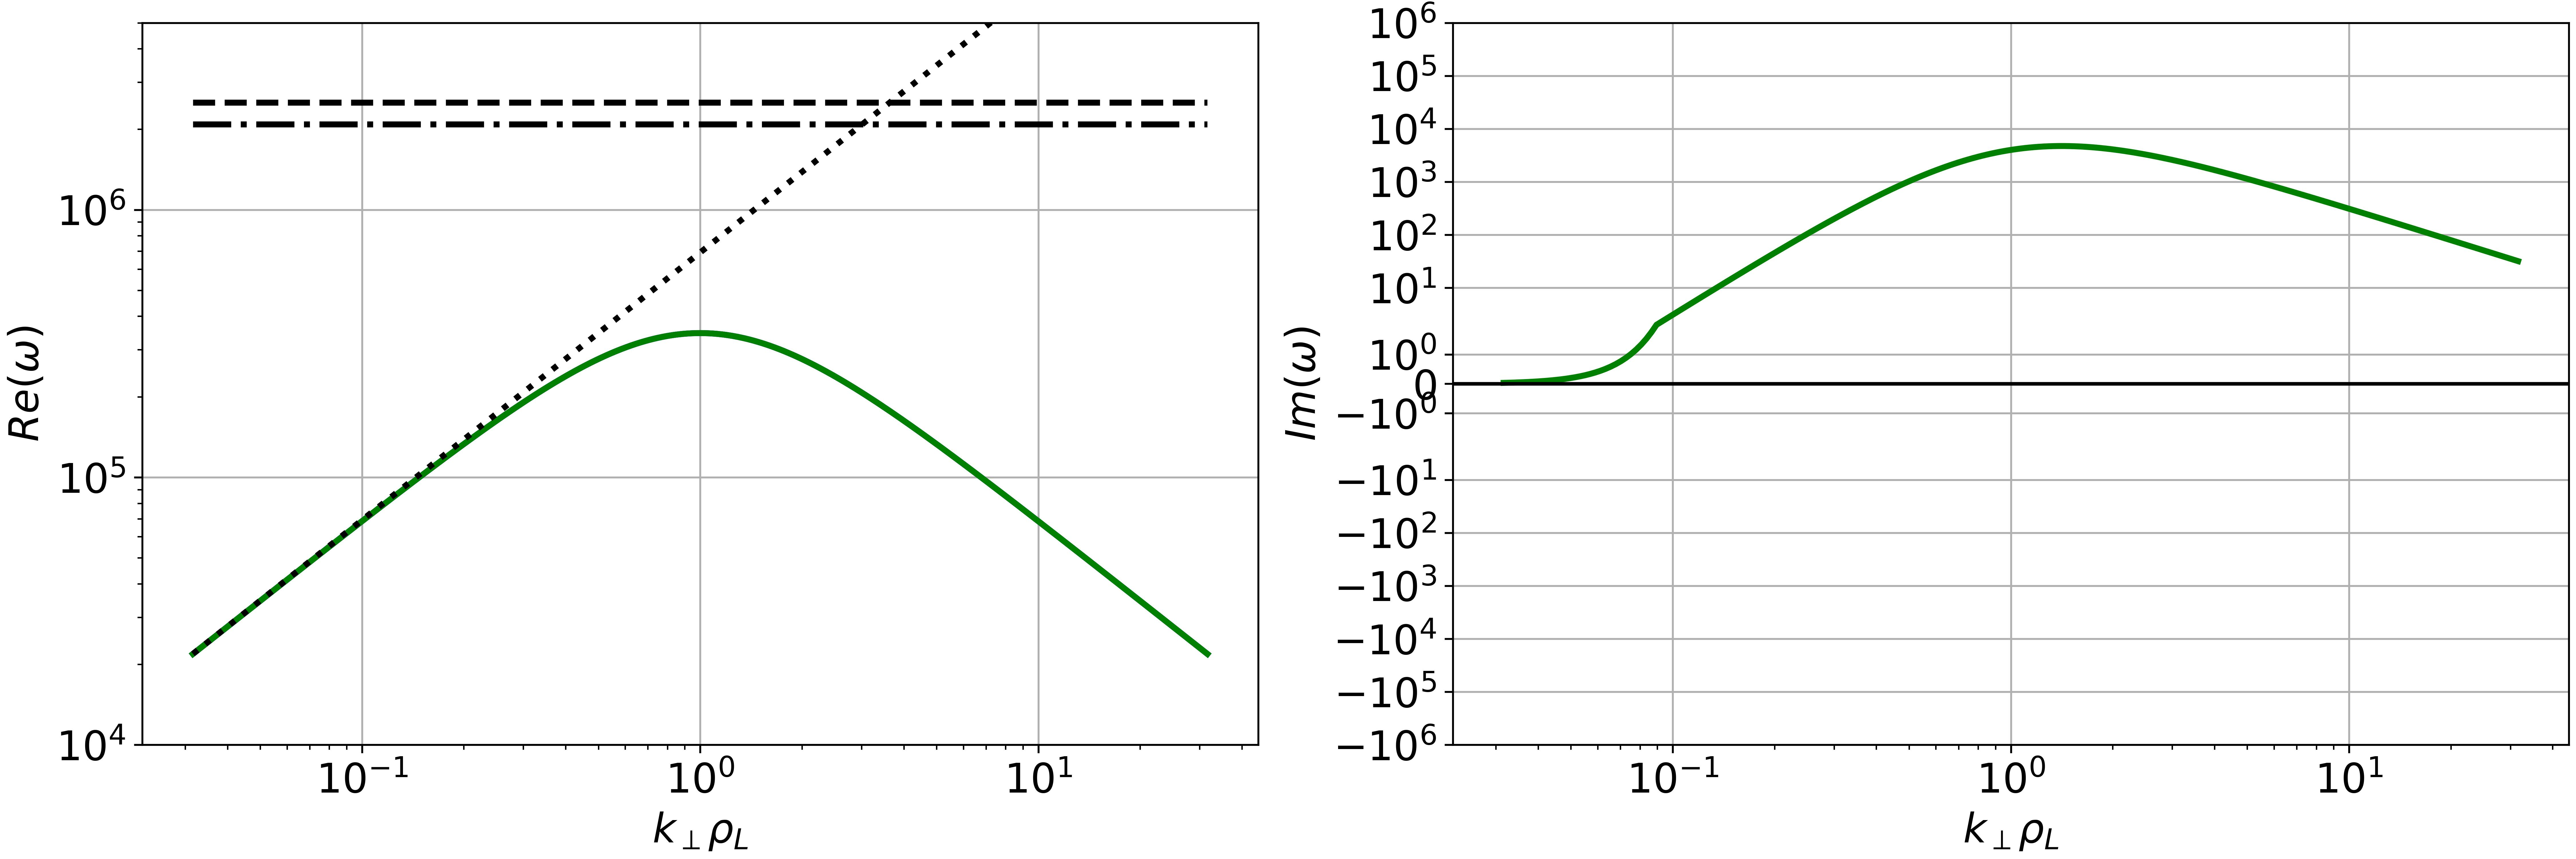
\includegraphics[width=1\textwidth]{schemes/modes_ES.jpg}
		\subcaption{Electrostatic system}
		\label{fig:anal_modesES}
	\end{subfigure}
\end{figure}
\begin{figure}[H]
	\ContinuedFloat
	\centering
	\begin{subfigure}[t]{0.85\textwidth}
		\centering
		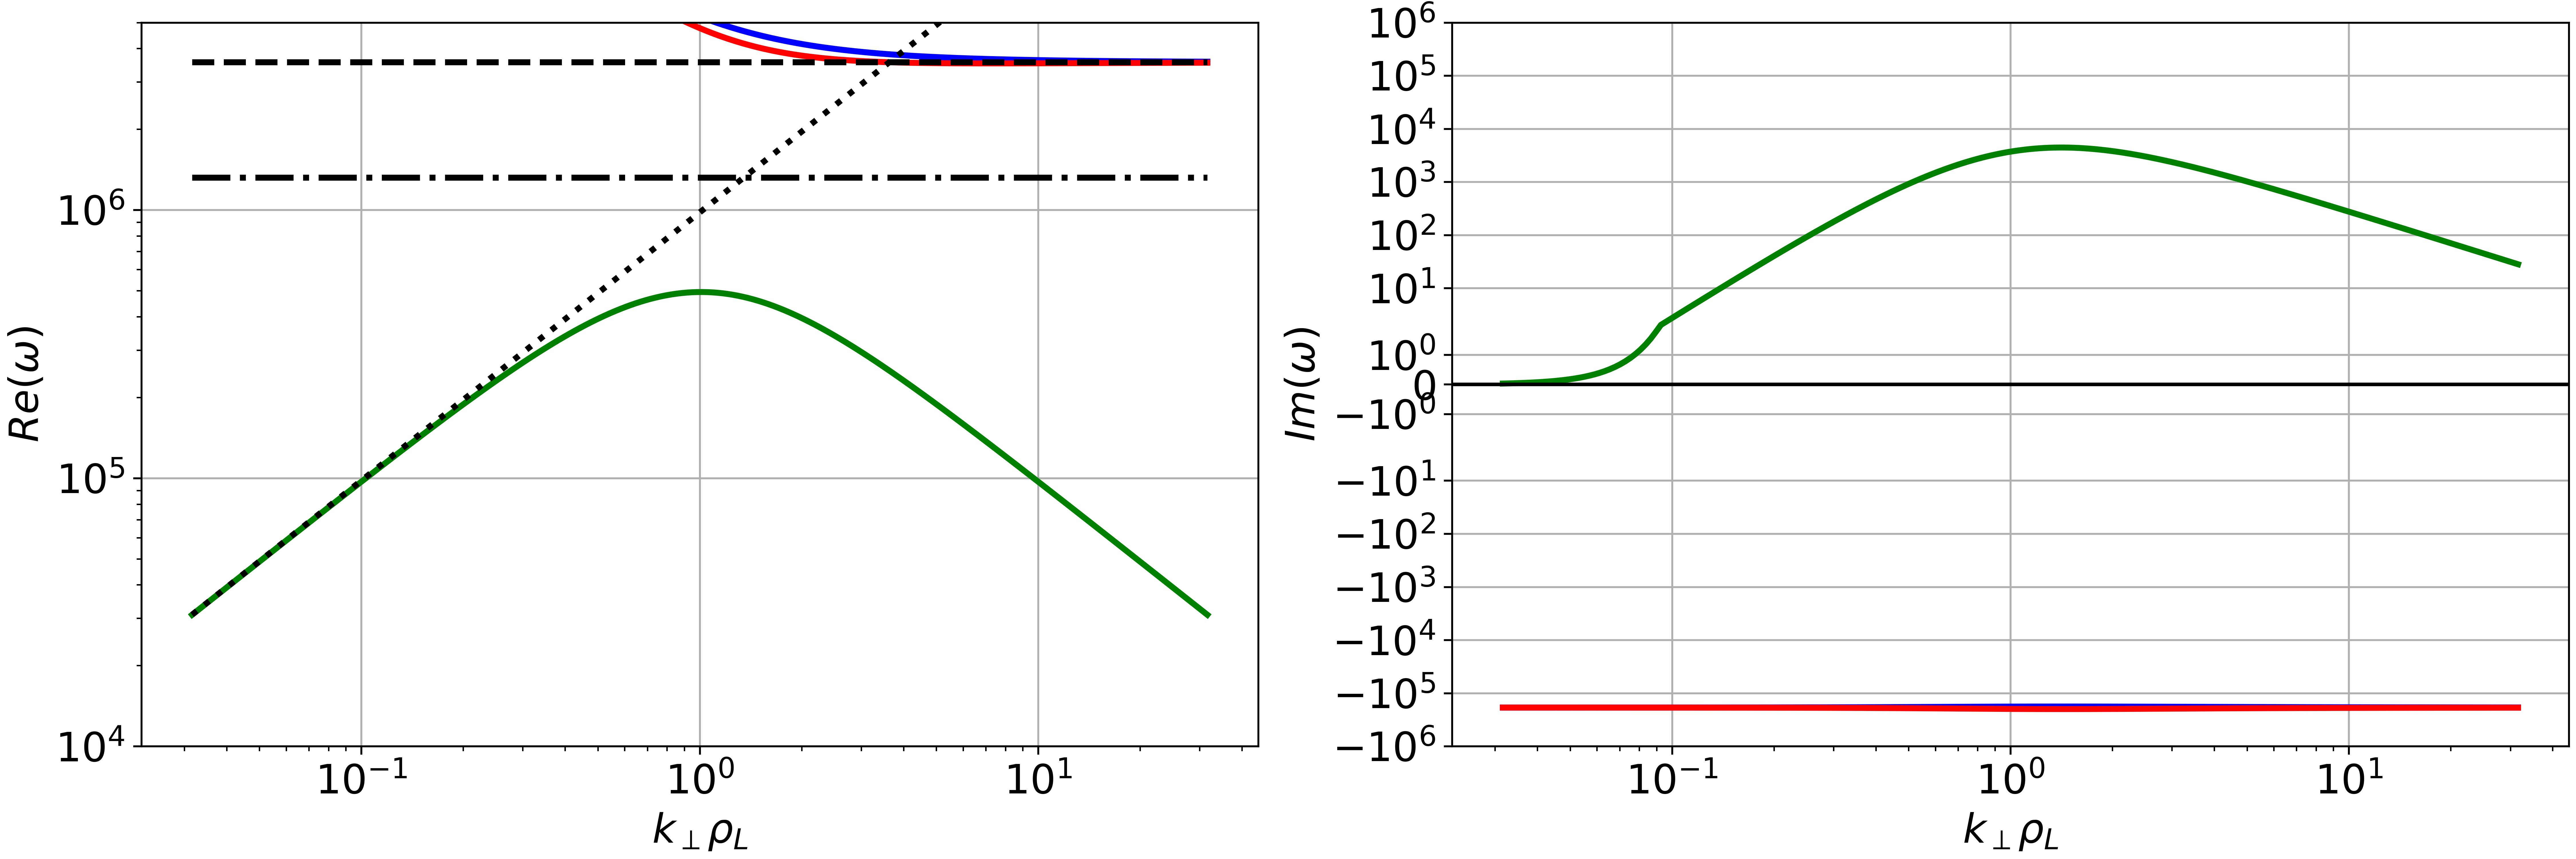
\includegraphics[width=1\textwidth]{schemes/modes_ES-inert.jpg}
		\subcaption{Electrostatic system with electron inertia}
		\label{fig:anal_modesEI}
	\end{subfigure}
\end{figure}
\begin{figure}[H]
	\ContinuedFloat
	\centering
	\begin{subfigure}[t]{0.85\textwidth}
		\centering
		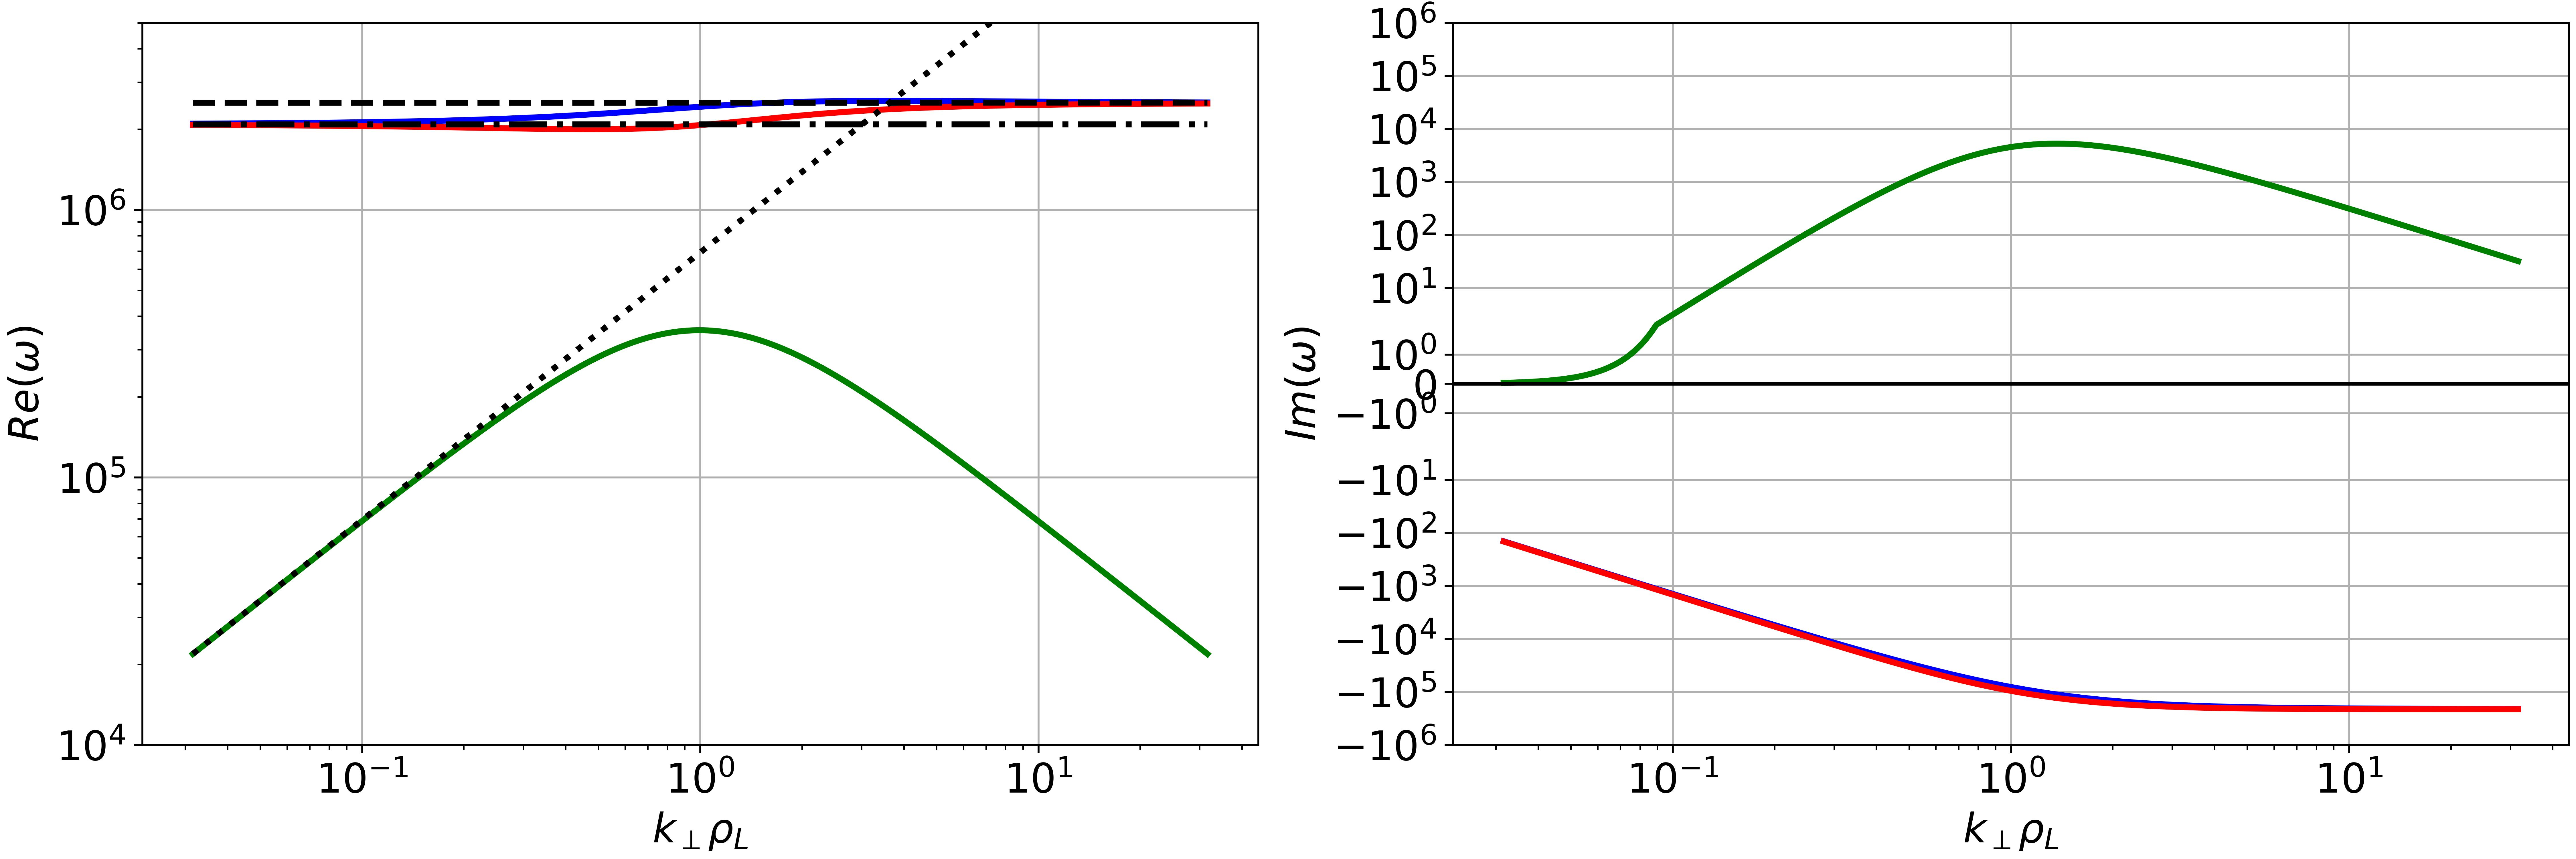
\includegraphics[width=1\textwidth]{schemes/modes_EM.jpg}
		%		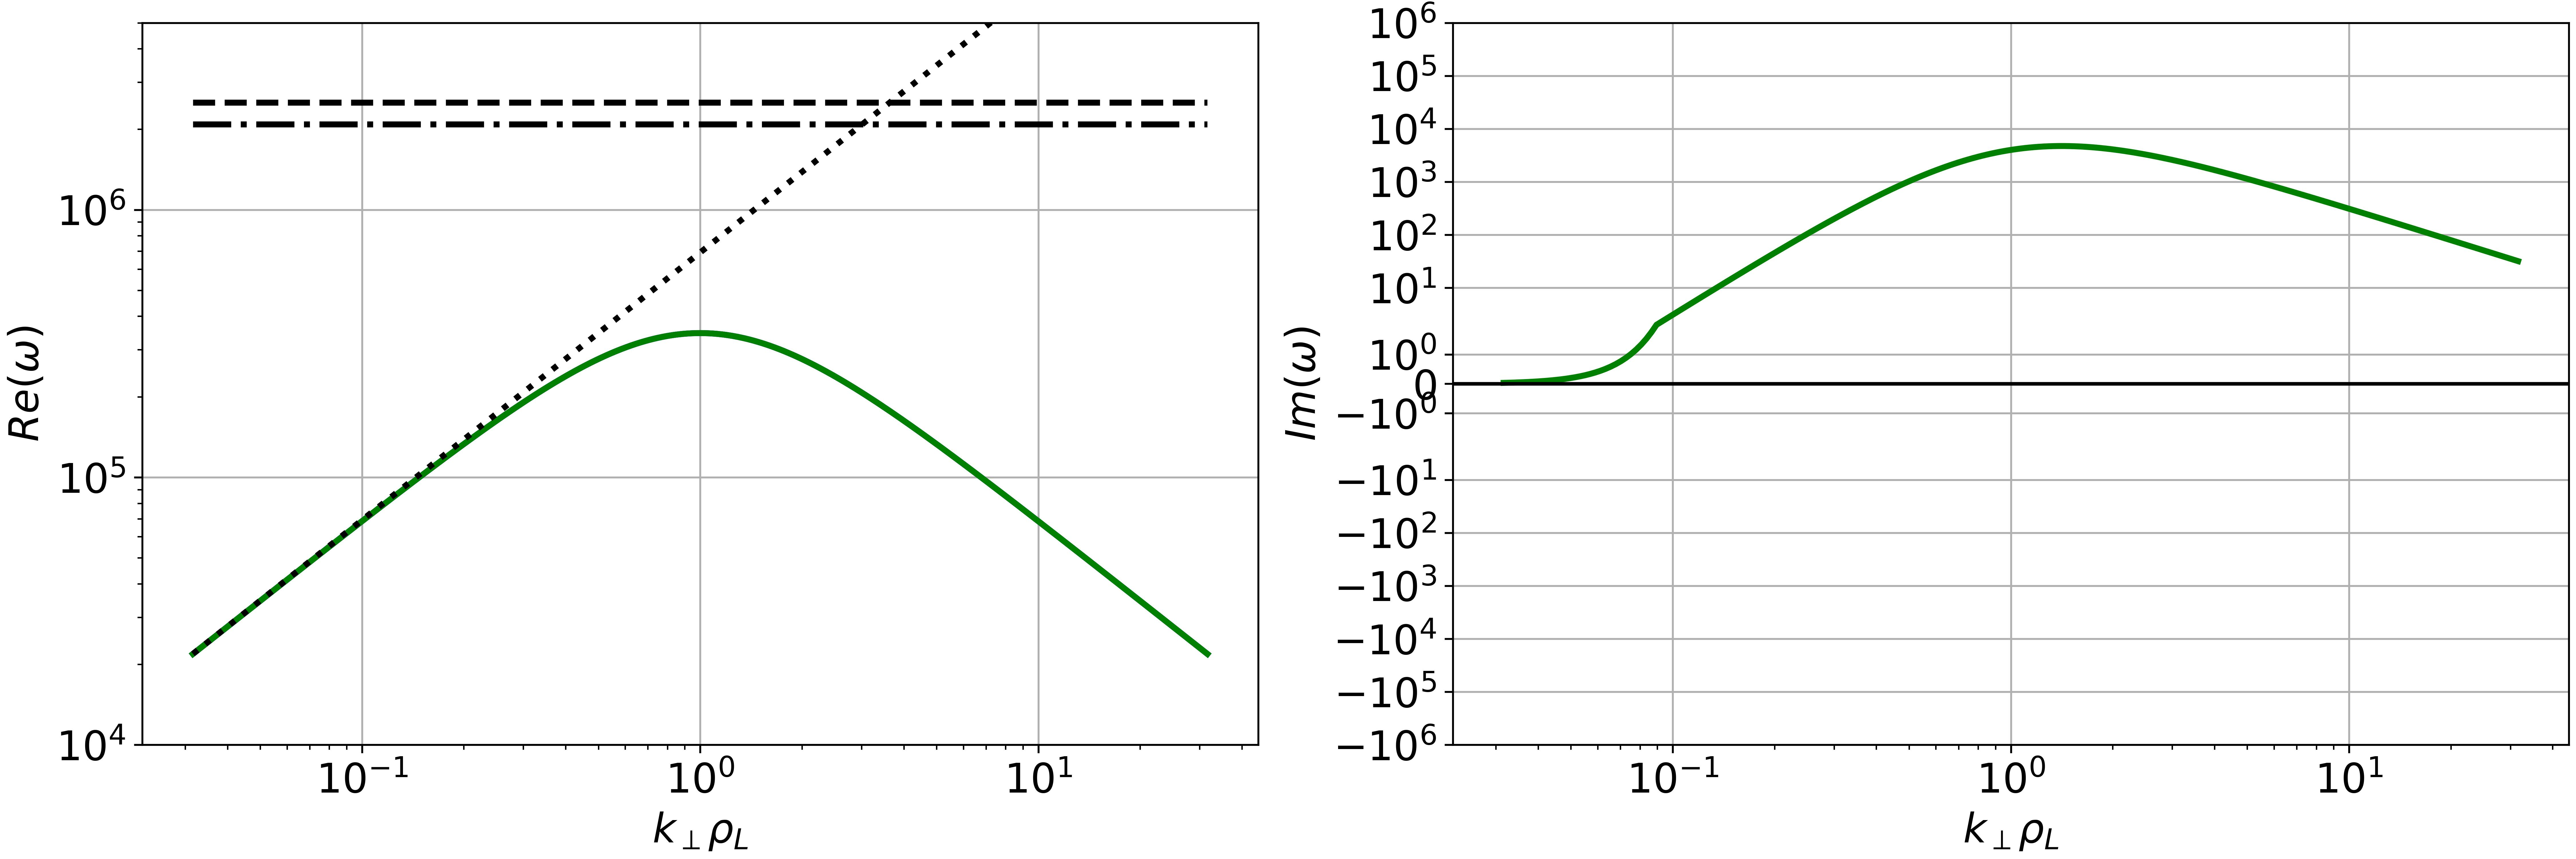
\includegraphics[width=1\textwidth]{schemes/modes_ES.jpg}
		\subcaption{Electromagnetic system}
		\label{fig:anal_modesEM}
	\end{subfigure}
\end{figure}
\begin{figure}[H]
	\ContinuedFloat
	\centering
	\begin{subfigure}[t]{0.85\textwidth}
		\centering
		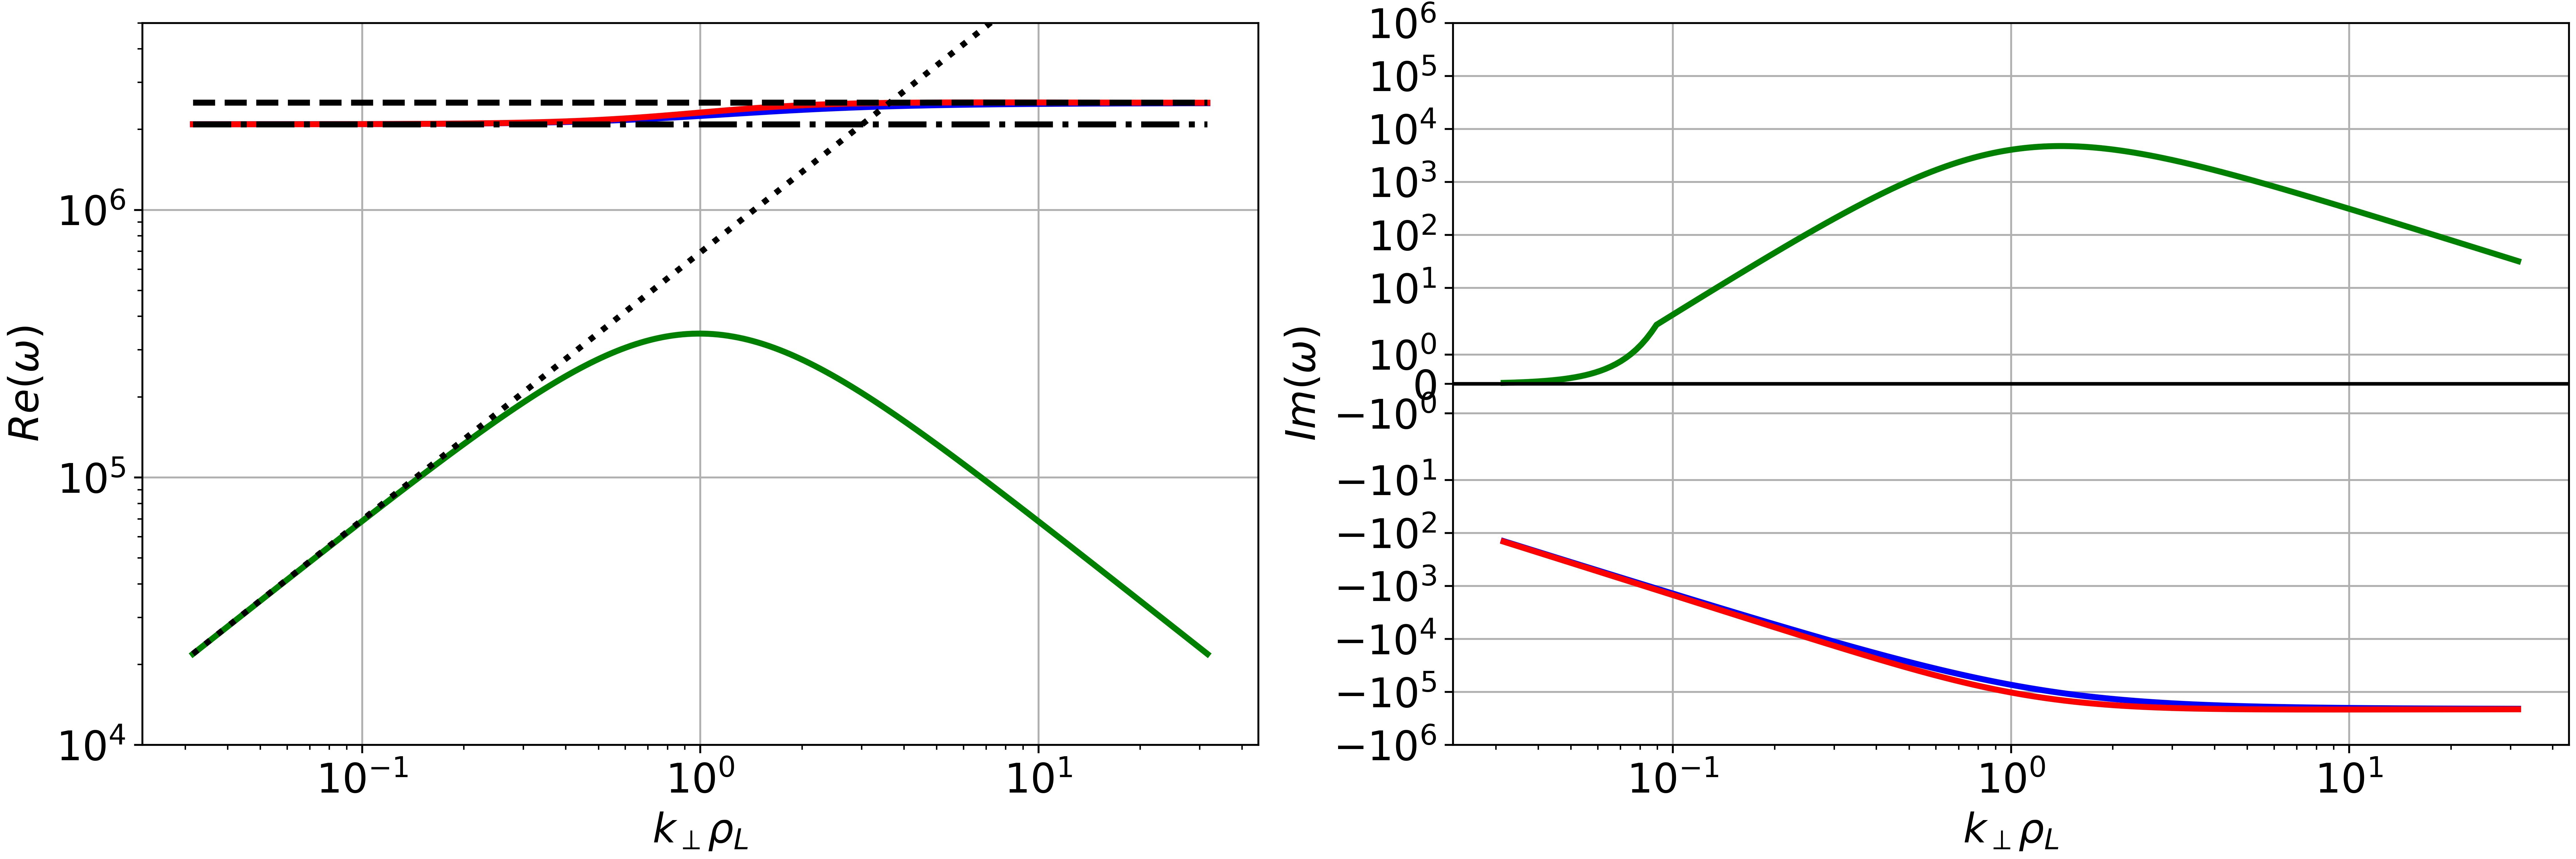
\includegraphics[width=1\textwidth]{schemes/modes_EM-flutter.jpg}
		\subcaption{Electromagnetic system with flutter}
		\label{fig:anal_modesFlutter}
	\end{subfigure}
	\caption{Dependency on the perpendicular wavenumber $k_\perp$ of the real and imaginary parts of the all solutions $\omega$ to the dispersion relation \ref{eq:anal_DAWdispersionRelation}. Except for $k_\perp$, all other values derive from: $B = 1$T, $n = 2\cdot10^{19}$m$^{-3}$, $T = 100$eV, $\lambda_p = 0.1$m and $k_\parallel = 0.6$m$^{-1}$. On a pair of graphs, a given color represents the same mode. In the left plots for $\Re{\omega}$, characteristic frequencies of the system are shown for reference ("--" diamagnetic $\omega_*$,"$\cdots$" electron sound $\omega_{s,e}$, "-$\cdot$-" Alfvén $\omega_A$).} 
	\label{fig:anal_modalBehavior}
\end{figure}

In the green curve, we observe the characteristic drift-wave frequency, which initially follows the diamagnetic frequency $\omega_*$ in the lower $k_\perp$ limit and reaches its maximum at $k_\perp \rho_L = 1$, before declining again. When the electron inertia term is introduced, a new mode emerges, starting at a significantly higher frequency before stabilizing at the electron sound frequency $\omega_{s,e} = v_{th,e} k_\parallel$. The introduction of electromagnetic terms governs the behavior of the new modes in the lower $k_\perp$ limit, which are then bounded by the shear Alfvén phase velocity. Qualitatively, the phase frequencies exhibit similar characteristics with or without flutter, with the primary difference being a more pronounced separation between the two modes as they transition from $\omega_A$ to $\omega_{s,e}$ in the pure induction. Overall, the characteristic frequencies of the electromagnetic modes are several orders of magnitude higher than the drift-wave frequency.

Looking at the growth rates associated with the modes, we first observe that drift waves are unstable with strong positive growth rates where the frequency is maximal, consistent with the earlier discussion about drift-wave instabilities. On the other hand, electromagnetic (and electron inertial) modes are very stable, showing strong negative $\gamma$. If one intends to study the growth and propagation of turbulent structures and their global impact, Alfvénic modes will only marginally contribute. It is hence possible to avoid the numerical costs involved with the high-frequency modes without much loss of accuracy.

It is more important to consider the effects of electromagnetic contributions on the drift-wave mode. For this purpose, Fig. \ref{fig:anal_comparisonDW} compares the real and imaginary parts of the drift-wave modes in the three electromagnetic scenarios with those in the electrostatic scenario.

\begin{figure}[H]
	\centering
	\begin{subfigure}[t]{0.45\textwidth}
		\centering
		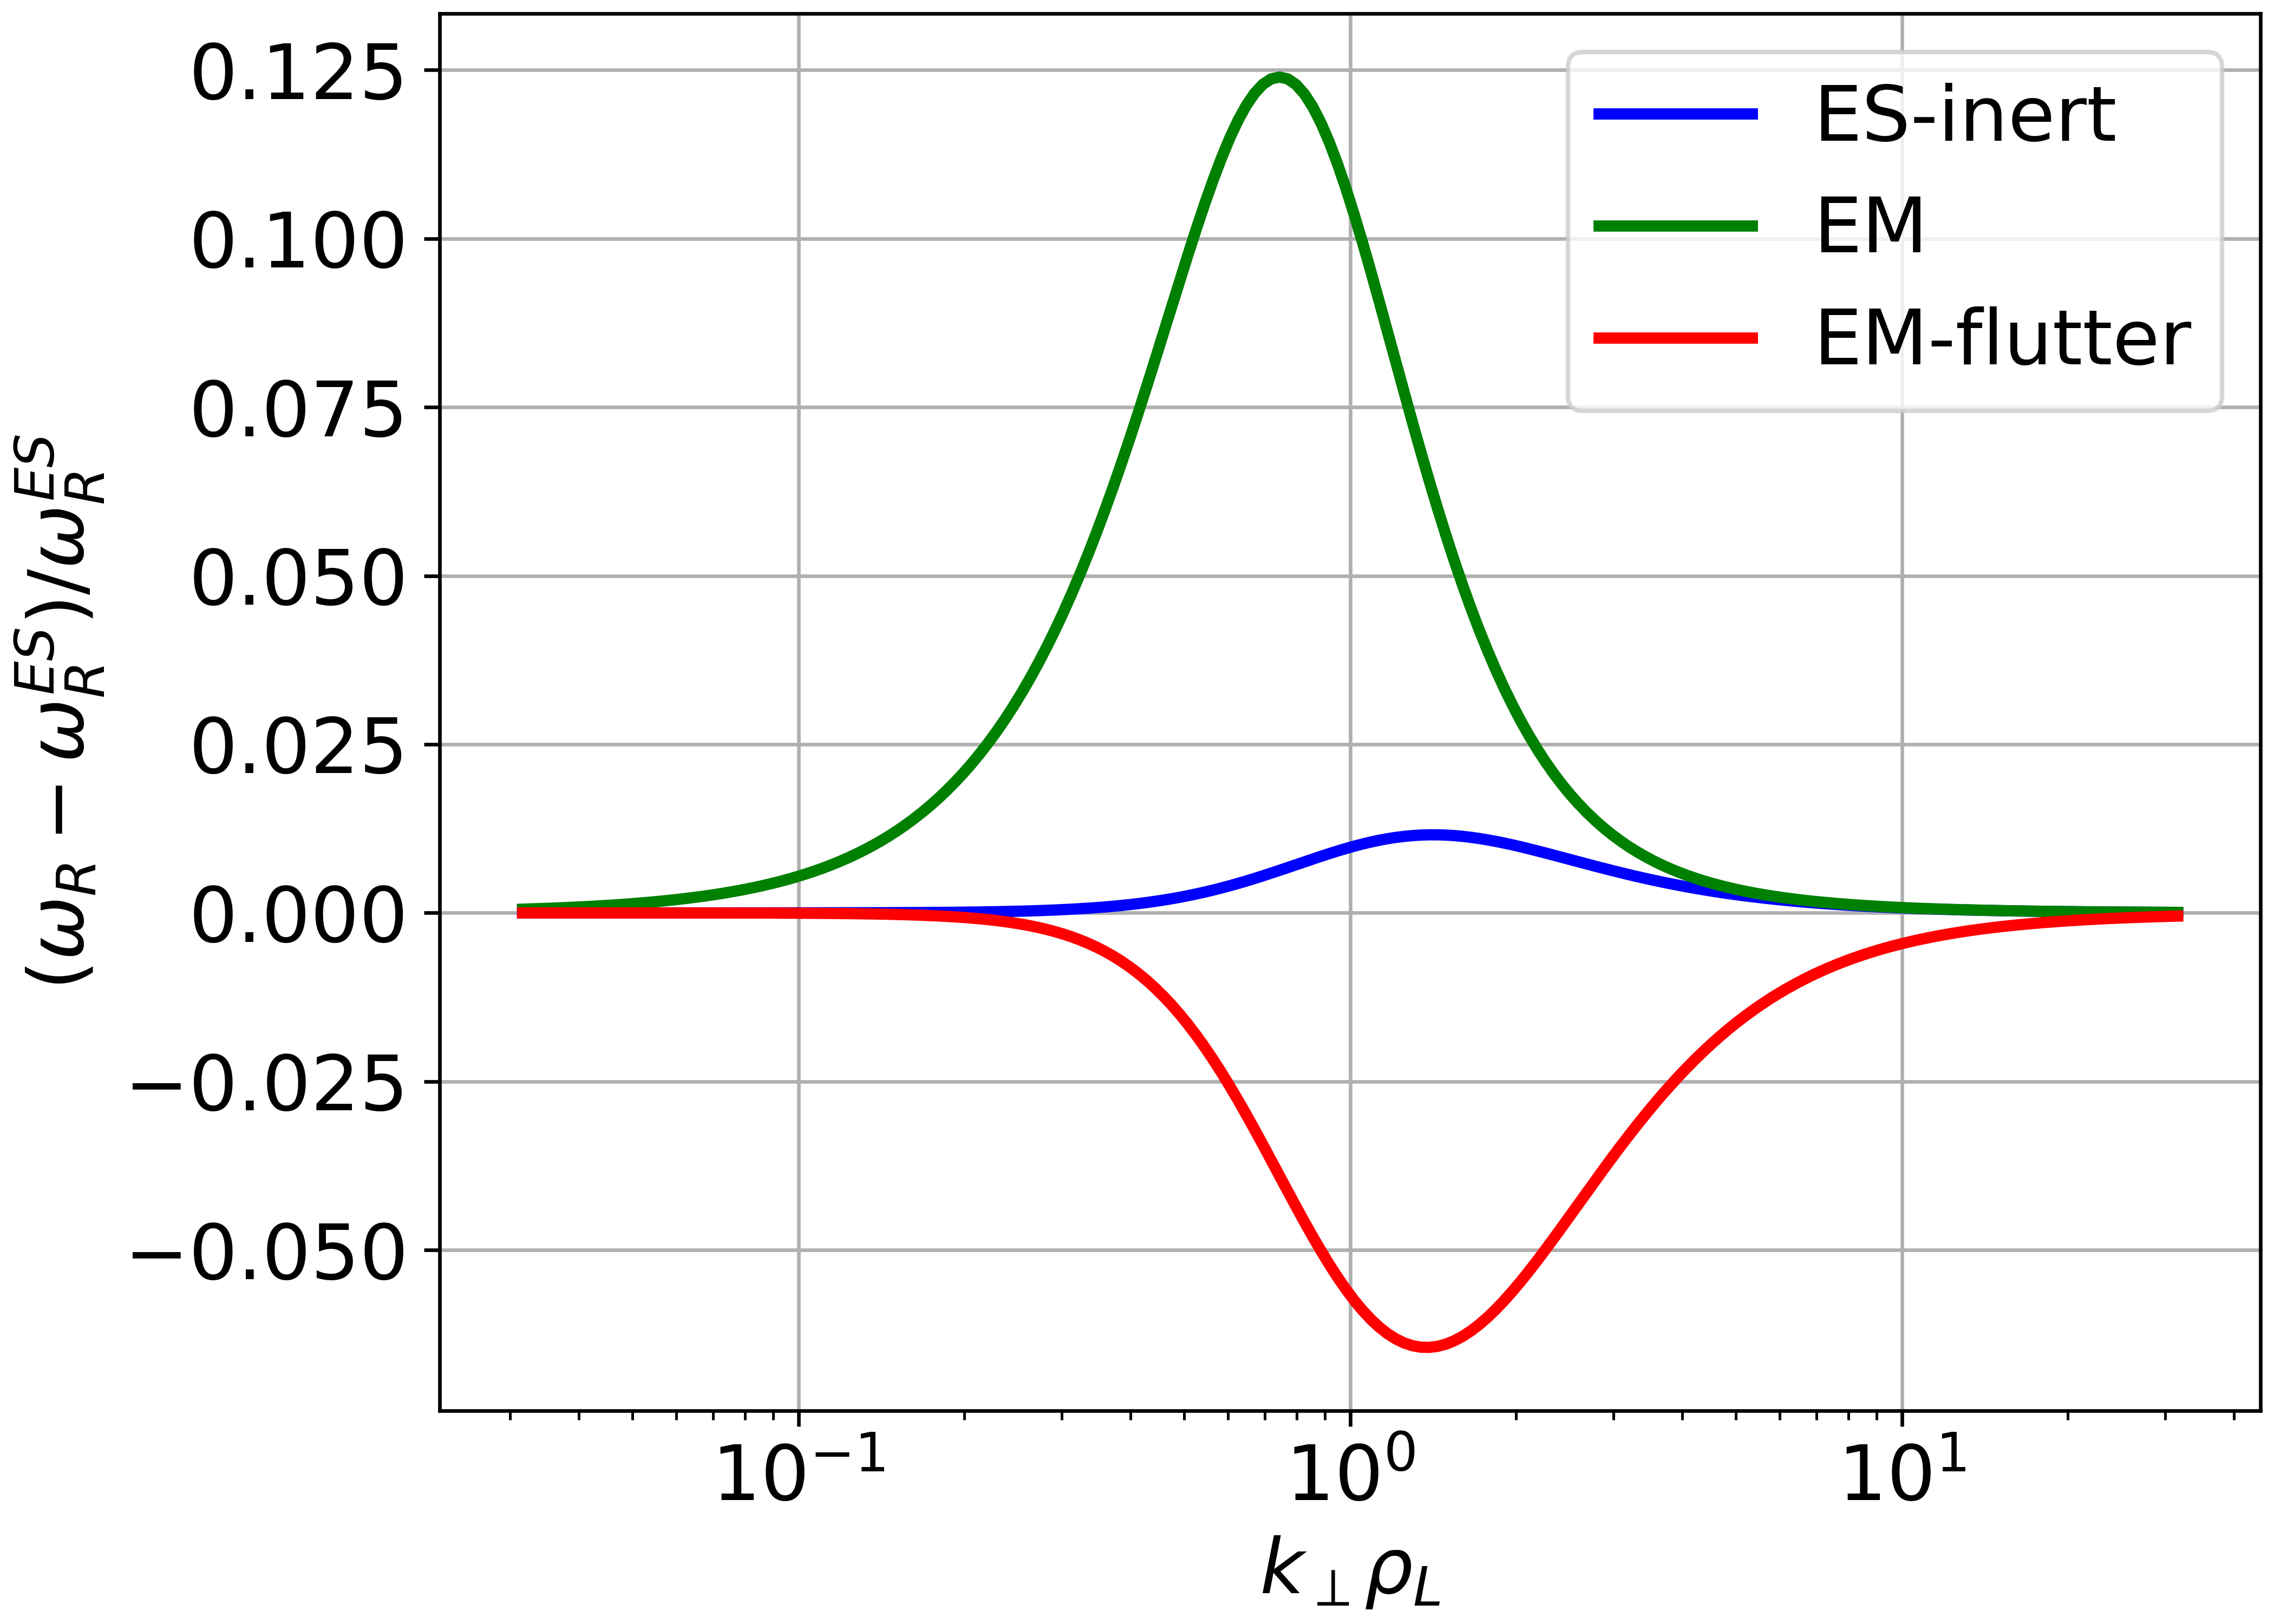
\includegraphics[width=1\textwidth]{schemes/comparison_DW_real.png}
		\subcaption{Real component}
		\label{fig:anal_comparisonDWreal}
	\end{subfigure}
	\begin{subfigure}[t]{0.45\textwidth}
		\centering
		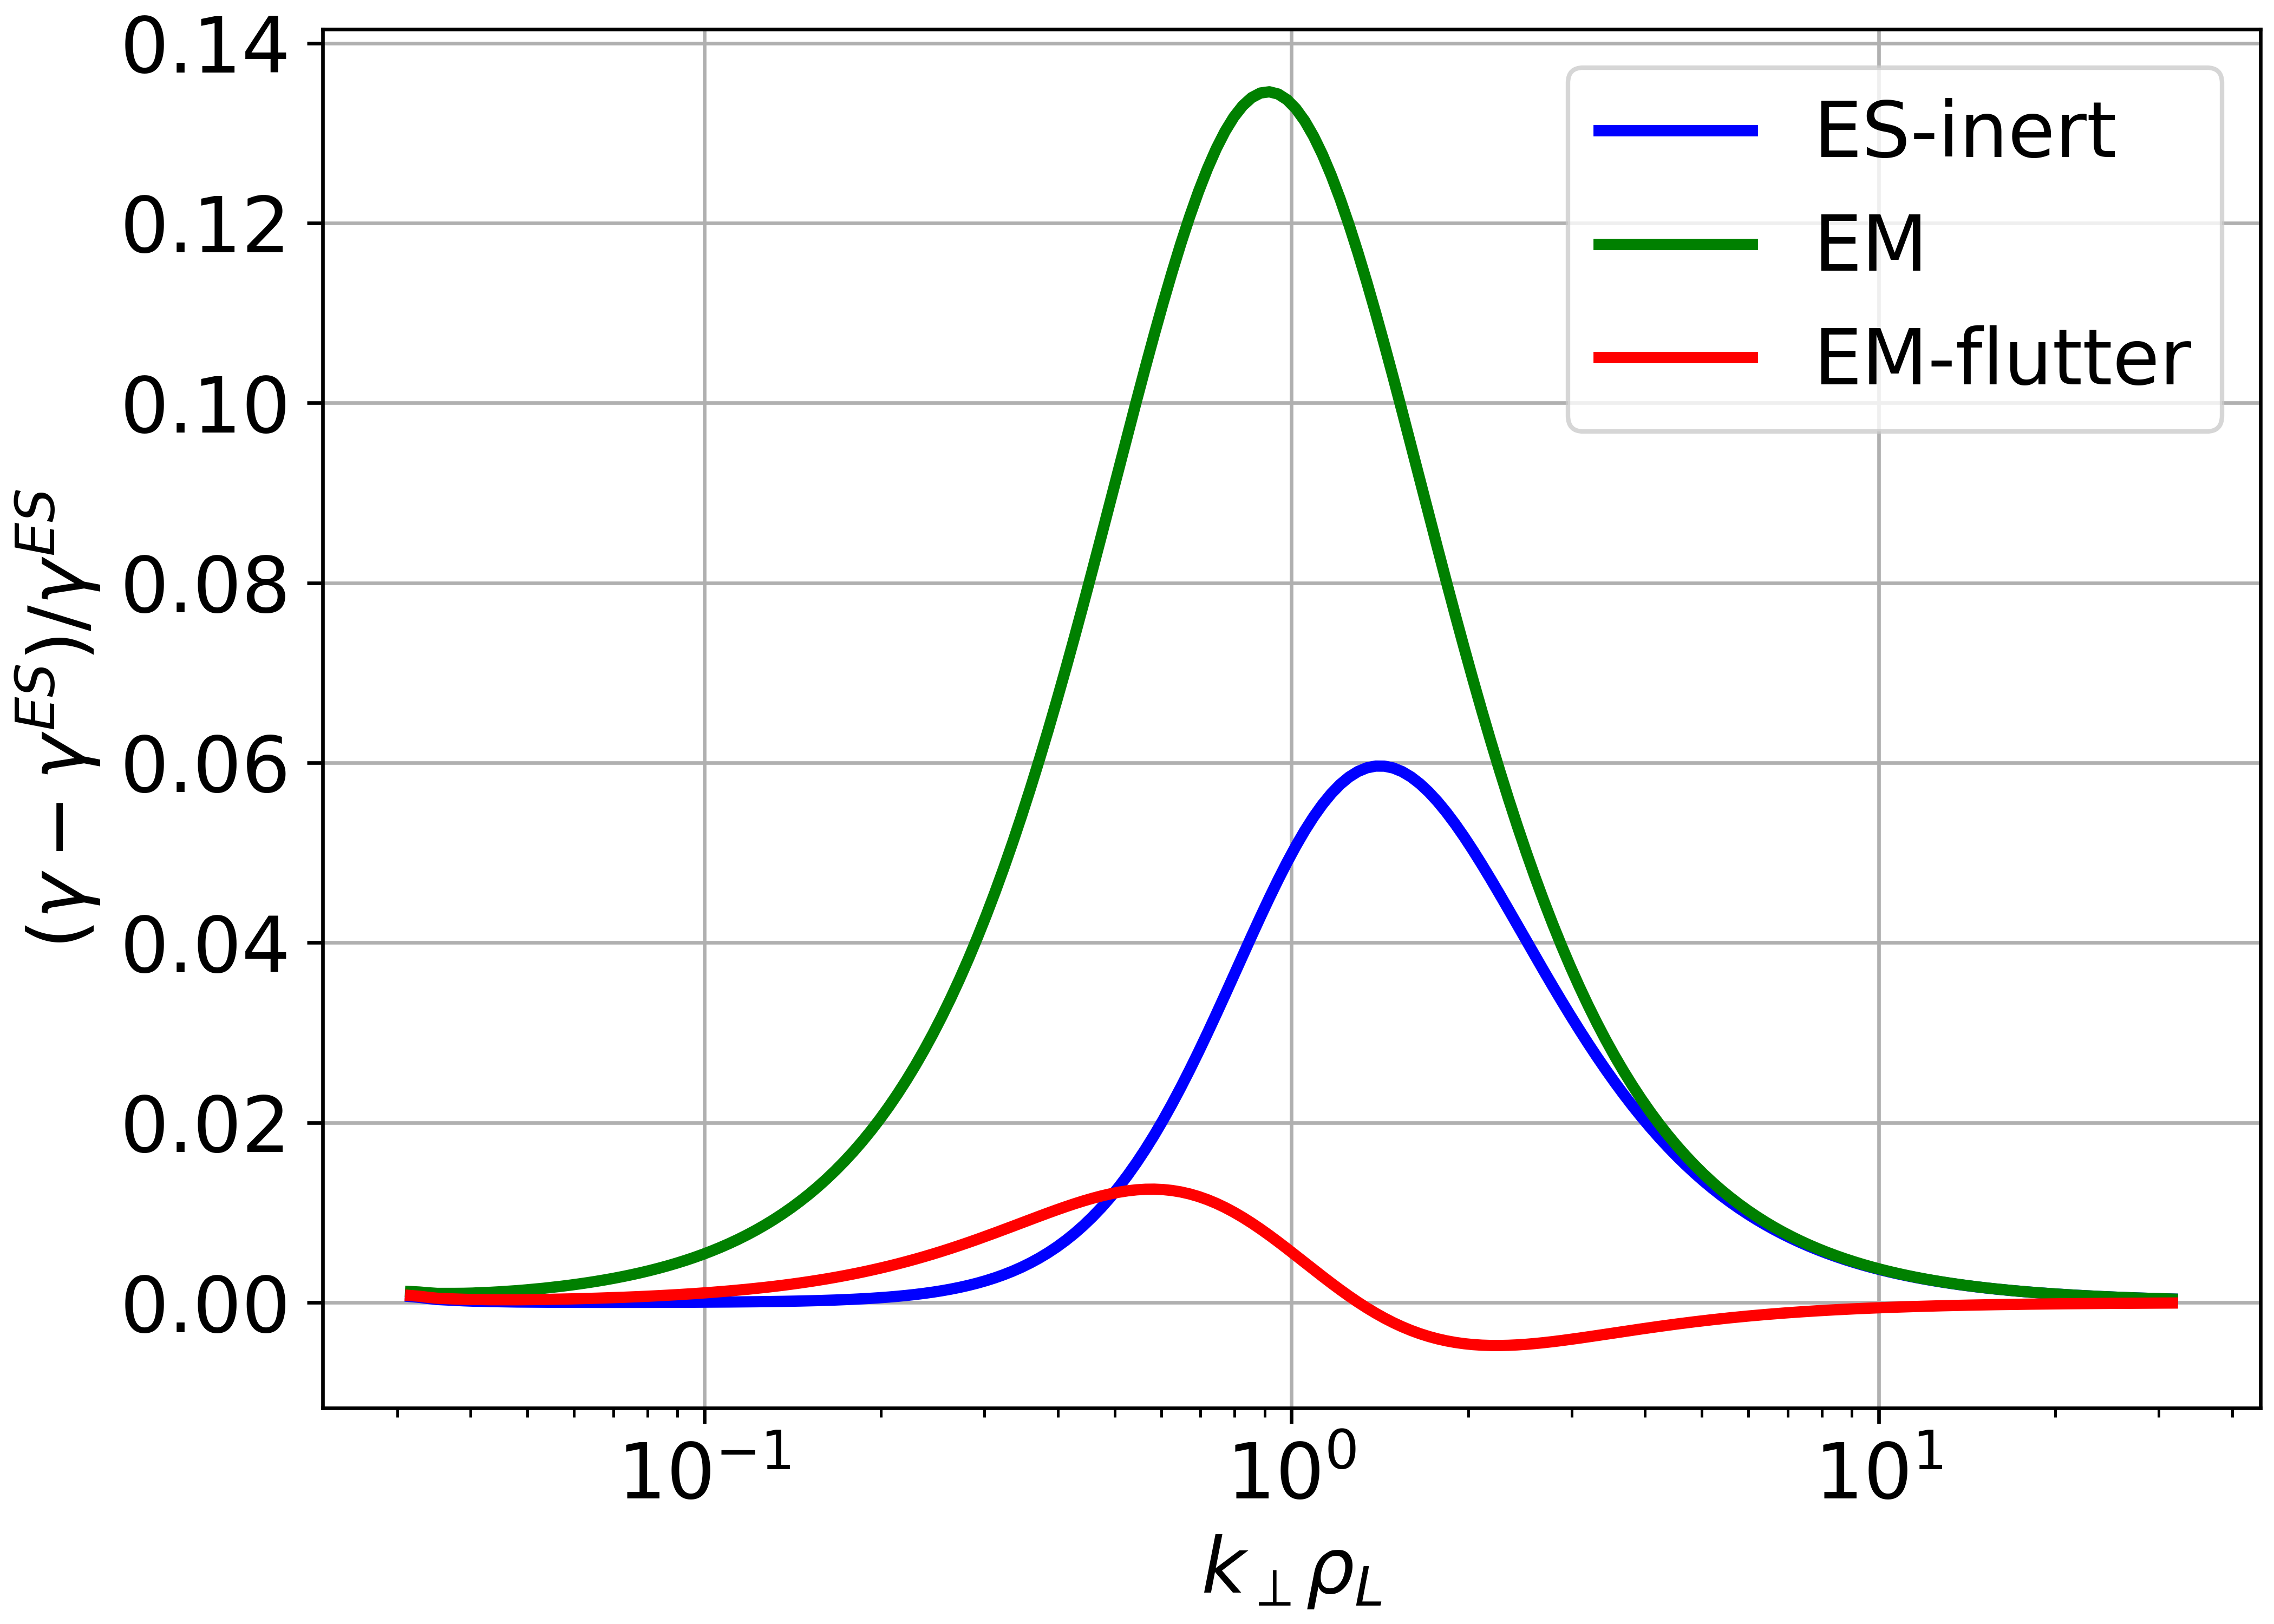
\includegraphics[width=1\textwidth]{schemes/comparison_DW_imag.png}
		\subcaption{Imaginary component}
		\label{fig:anal_comparisonDWimag}
	\end{subfigure}
	\caption{Relative difference of drift-wave frequency in the electromagnetic scenarios to the reference electrostatic case.} 
	\label{fig:anal_comparisonDW}
\end{figure}

The real part is altered by the electromagnetic additions, but the change of phase frequency will only have a minor impact on production cases. On the other hand, the growth rate increases with electron inertia and even more with electromagnetic induction. Electromagnetic flutter on the other largely mitigates the instabilities, and can even reduce the growth rate observed in electrostatic drift waves.



\section{Slab configurations}
\subsection{Analysis of a plasma blob}
\label{ssec:plasmablob}

The linear analysis from the previous section has only , as characteristic shear Alfvén and thermal electron times are much shorter than the ion cyclotronic time, which underlies the resolution of typical turbulent SOLEDGE3X simulations. Drift Alfvén waves in turn correspond to the impact of inductive electromagnetic effect on the formation of drift waves, where the term $\partial_t A_\parallel$ in Ohm's law modifies the non-adiabatic response of the potential $\Phi$ to parallel fluctuations of the electron pressure $p_e$. To study the these effects on a plasma blob in a slab domain. \newline

We place ourselves in a plasma environment similar to the separatrix region in the diverted TCV simulations from the next Chapter \ref{chap:TCV}. The magnetic field is aligned to the toroidal coordinate with $B_{eq,t} = 1.3$T with a curvature of $1.1$m from the tokamak center, similar to the position of the separatrix at the outer mid-plane in TCV. Limiters are placed at both toroidal ends such that that connection length $L_\varphi = 65$m. A cartesian grid with coordinates $r$ and $z$ discretizes each poloidal plane, allowing radial fluxes out and with periodic boundary conditions in the vertical $z$-direction. The electron temperature is kept constant at $T_e=60$eV, ions are cold and the background density is set to $n_0 = 10^{19}$part/m$^3$. To simplify the study and prevent numerical difficulties at the sheath, we apply Neumann-0 boundary $\partial_\parallel n^{BC} = 0$ on the density and the potential $\Phi$ is fixed to $\Phi^{BC} = \Lambda T_e^{BC}$. This is a major simplification to the typical SOLEDGE3X sheath conditions described in Sec. \ref{sec:S3X_boundaryConditions}. The axisymmetric blob initially takes a Gaussian profile 

\begin{equation}
	n = n_0 \left(1 + \alpha e^{-\left[(r-r_b)^2+(z-z_b)^2\right]/\delta_b}\right)
	\label{eq:blobInitProfile}
\end{equation}

with a blob overdensity $\alpha = 2$ and radius $\delta_b = 1$cm. The blob evolves with curvature and electric drifts, neglecting anomalous perpendicular diffusion and viscous effects. Further, electron inertia effect are neglected with $m_e = 0$. We compare the reference electrostatic case with magnetic induction in the parallel electric field and the full electromagnetic setting including flutter. The simulation results are collected in Fig. \ref{fig:BLOB}. \newline

\begin{figure}[H]\centering
	\centering
	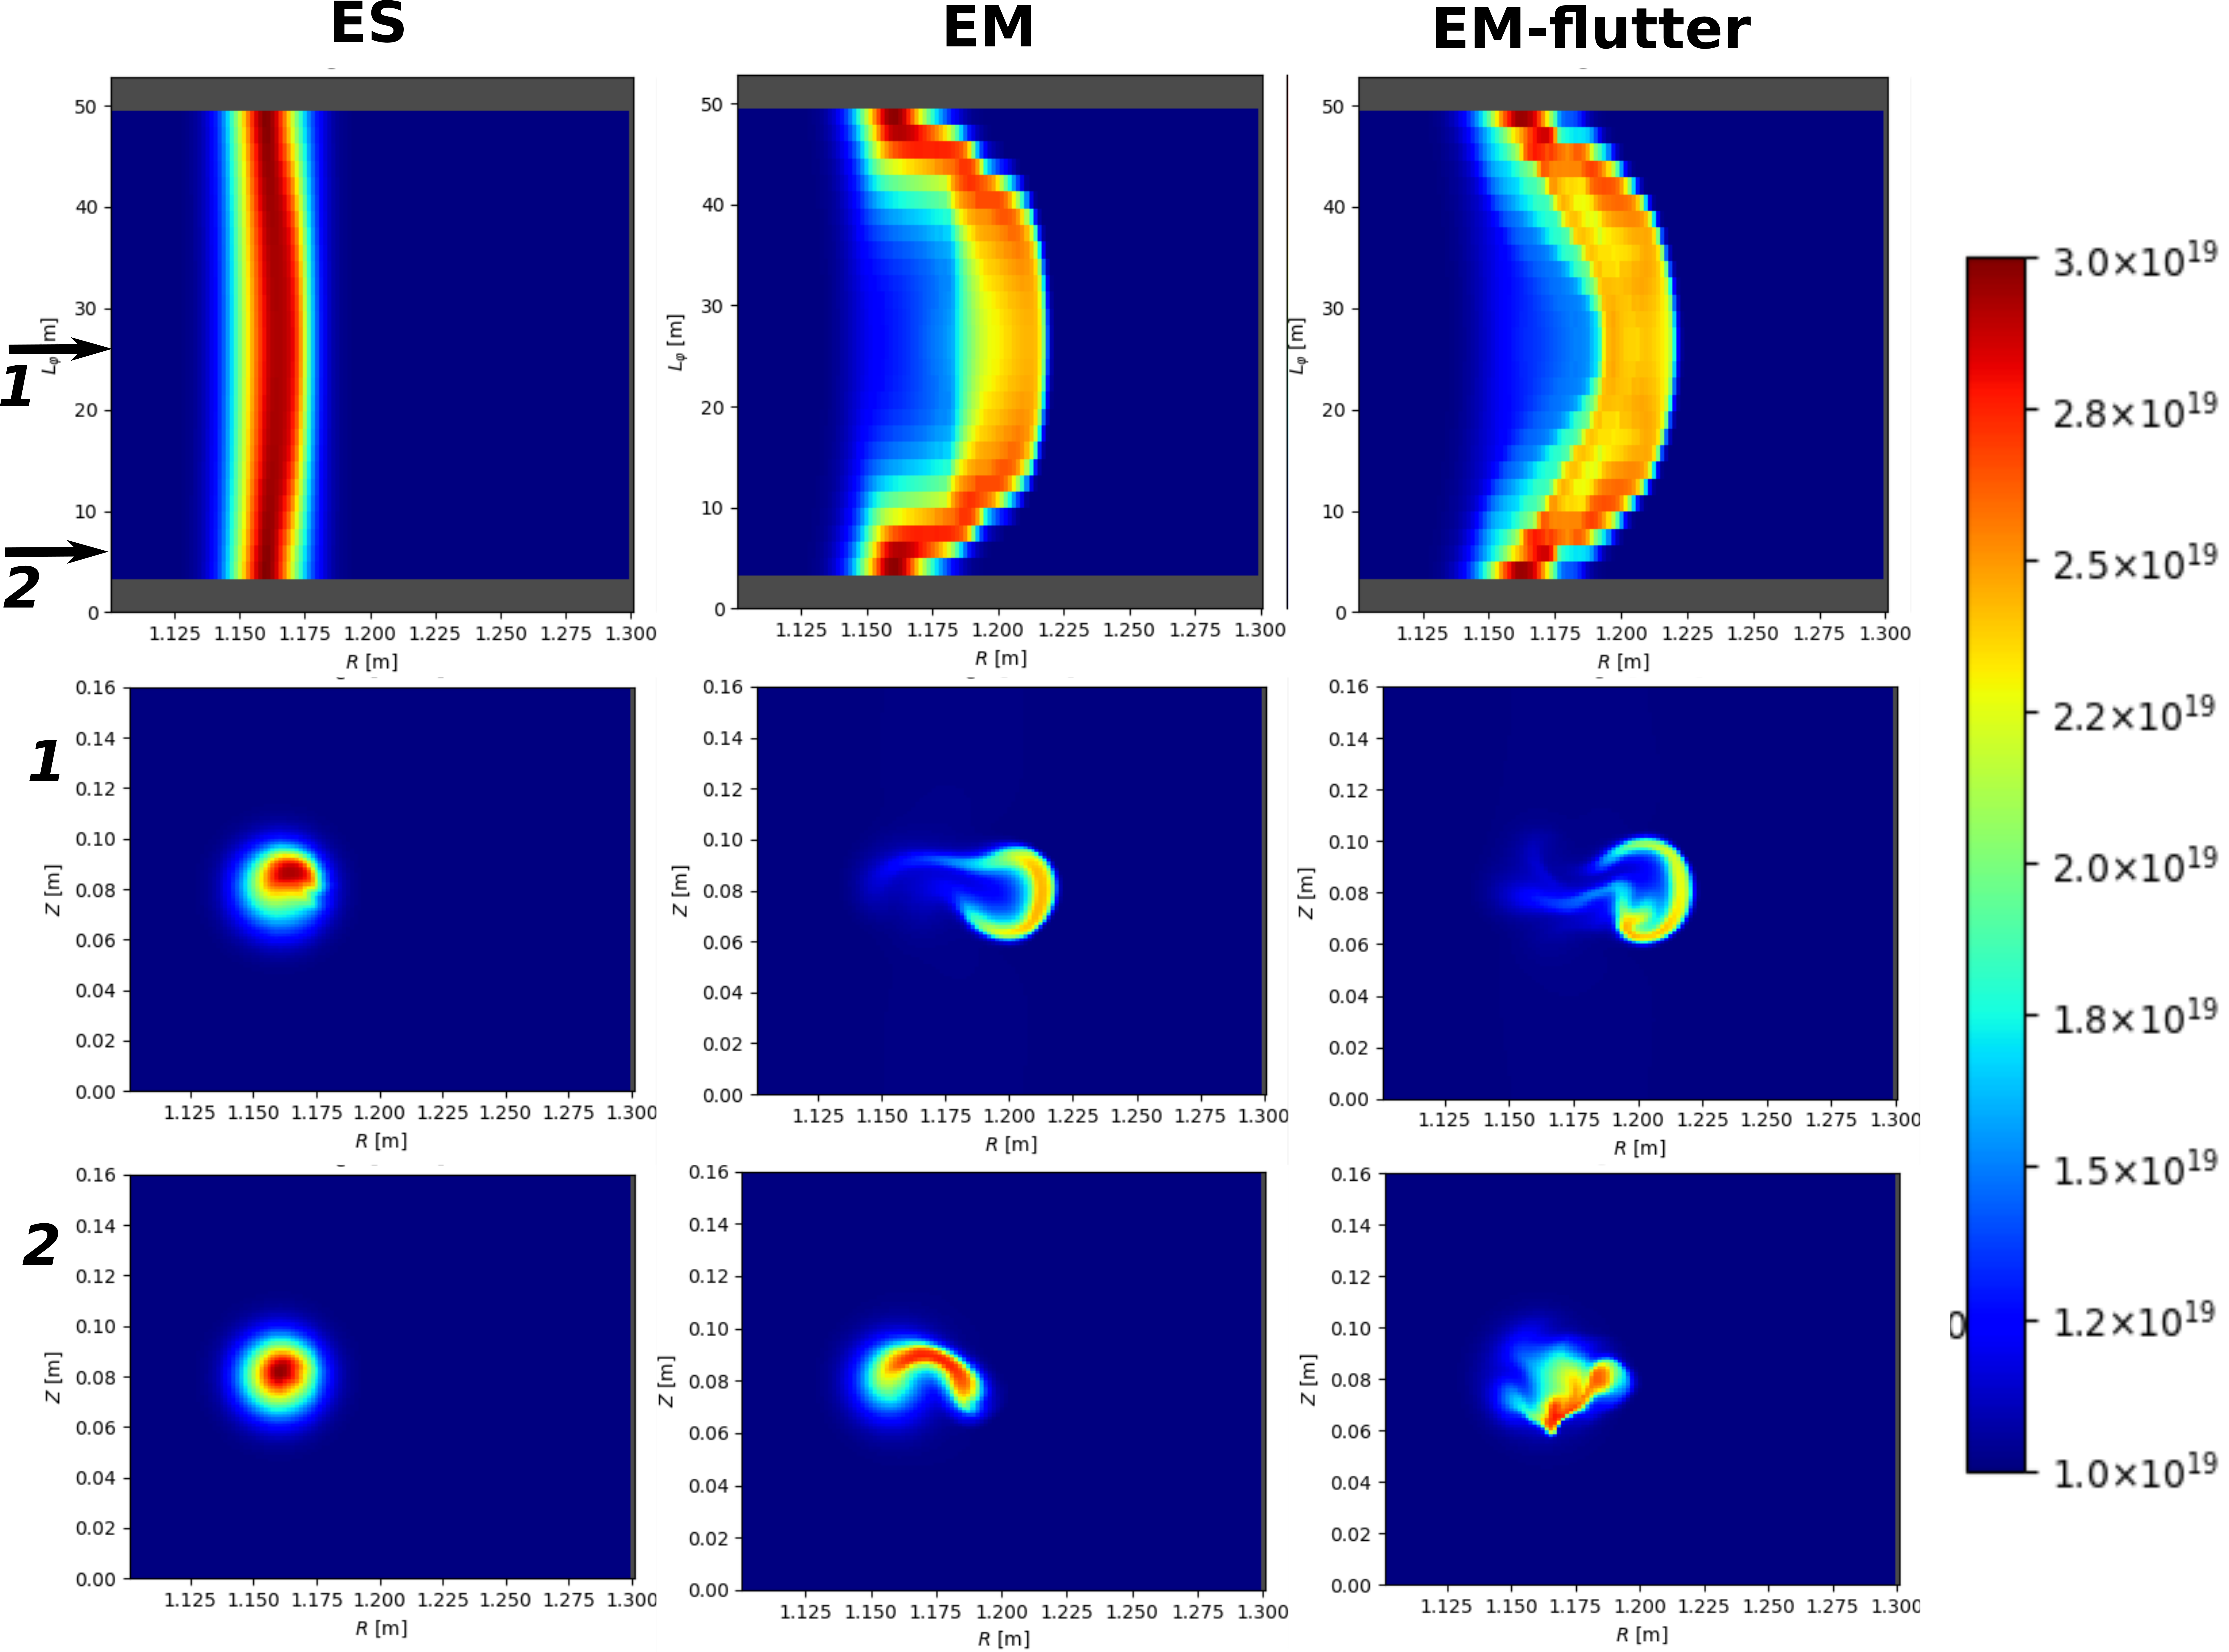
\includegraphics[width=1.\textwidth]{schemes/blob_compare_9_6_microsec.png}
	\caption{Density profiles [part/m³] after 9.6$\mu$s simulated plasma time for the electrostatic (ES), magnetic inductive (EM) and full electromagnetic scenarios (EM-flutter). The first row shows a view of the $R-\varphi$ plane with the maximum density taken along the $Z$ coordinate. The second and third rows show the density on poloidal planes ($R-Z$) at the center of the field lines (1) and in proximity to the sheath (2).}
	\label{fig:BLOB}
\end{figure}

In the center of the domain, drift waves determine the potential $\Phi$ but it is dominated by the sheath in proximity to the limiters. Hence a parallel gradient appears on $\Phi$, which in turn induces a parallel current responsive to inductive electromagnetic effects. As a result, the blob filaments bends along the toroidal direction, with higher advection velocities in the center of the domain than at the sheath. The bending is much more pronounced for the two electromagnetic scenarios, in line with the findings of previous blob studies\cite{lee2015,lee2015electromagnetic,Stepanenko_2020}. On closed field lines, the blob would conserve its axisymmetry and both $j_\parallel$ and $A_\parallel$ would remain 0 throughout the simulation. \newline




\subsection{Generation of drift waves}
\label{ssec:plasmaturbslab}

In the previous section, we examined how a single plasma blob propagates across open field lines. However, this does not account for how the blob appears in the first place. In this second part of the slab study, we investigate the onset of drift waves. We consider the same setting as before but with a background density of $n_0 = 2 \cdot 10^{19}$ part/m$^3$ and isothermal electrons and ions at $T_e = T_i = 50$ eV. Instead of an initial overdensity, we apply a constant particle source of $5 \cdot 10^{22}$ part/s on the core side, at all $R < 1.12$ m. The emergence of drift-wave instabilities for the three scenarios is shown in Fig. \ref{fig:SLABturb}. \newline

\begin{figure}[H]\centering
	\centering
	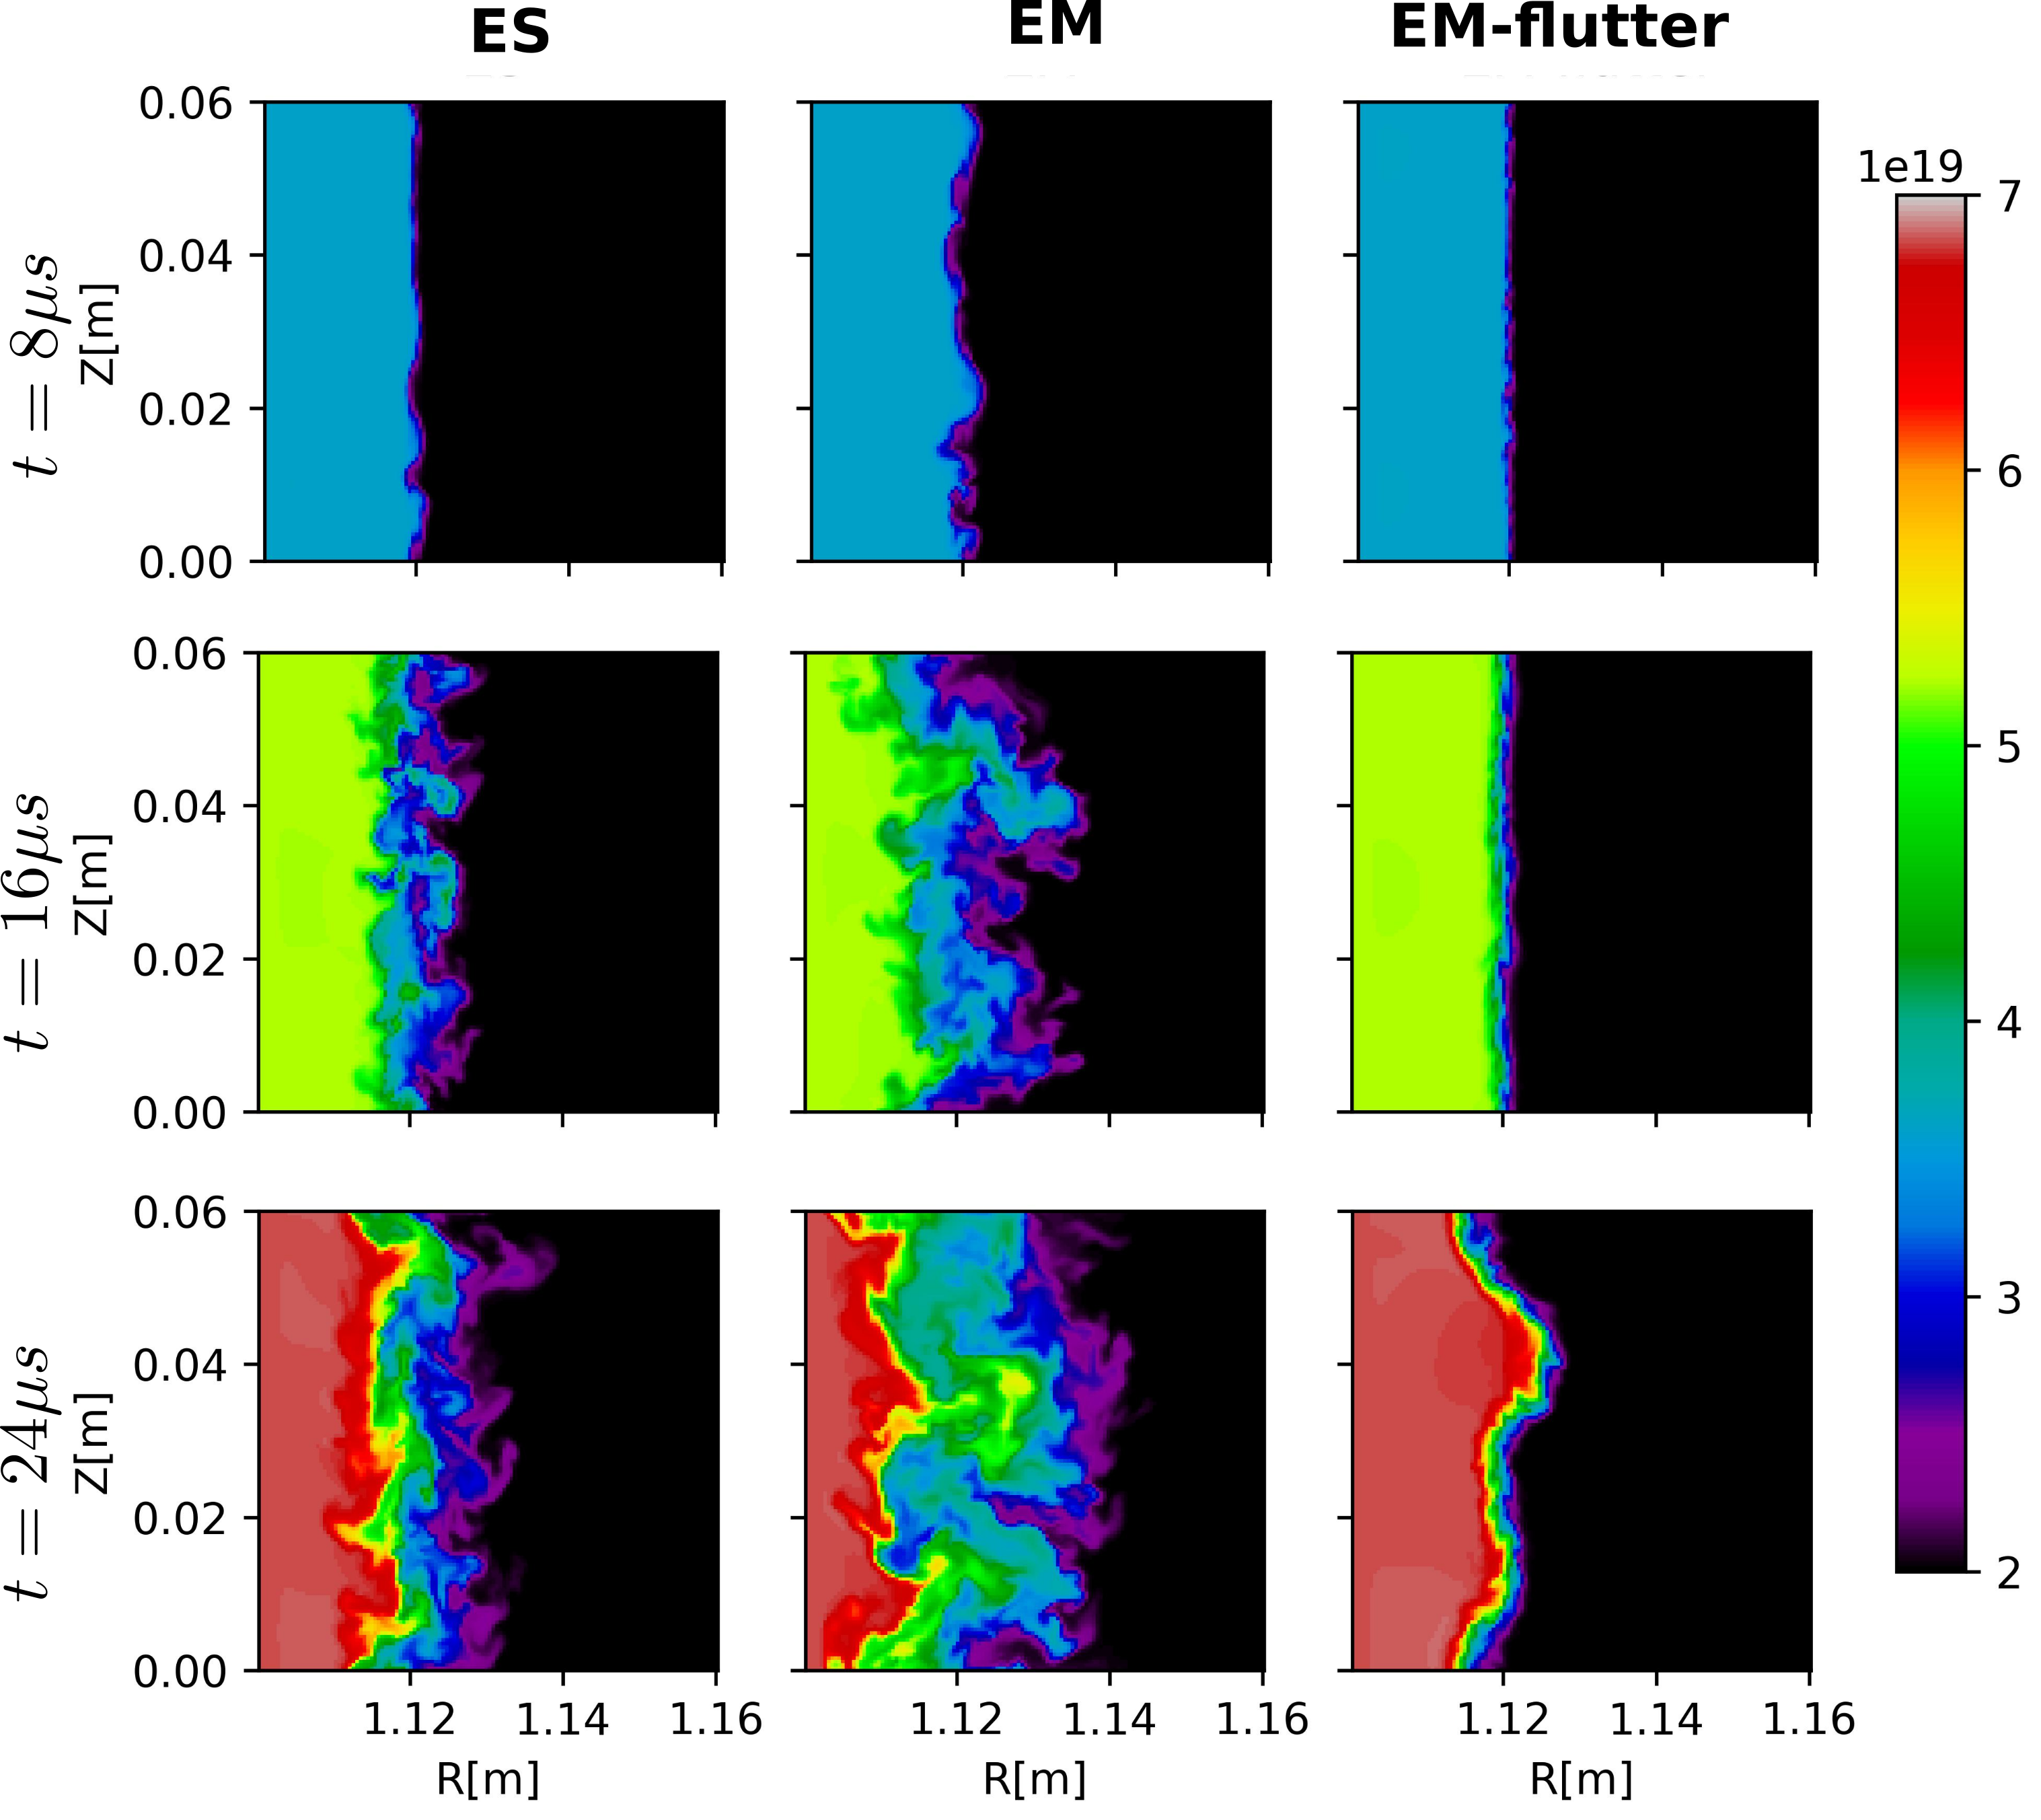
\includegraphics[width=.95\textwidth]{schemes/slab_source.png}
	\caption{Density profiles [part/m³] at the toroidal center of the slab, at about 32m from both limiters. The snapshots compare the electrostatic (ES), magnetic inductive (EM) and full electromagnetic scenarios (EM-flutter) scenarios after 8, 16 and 24$\mu$s simulated plasma time.}
	\label{fig:SLABturb}
\end{figure}

Initially, the particle source causes the density to build up on the core side of the slab. The radial gradient becomes stronger and soon collapses into drift waves. These waves are particularly pronounced in the electrostatic and electromagnetic inductive models. The term $\partial_t A_\parallel$ in Ohm's law intensifies the turbulent interchange, with plasma filaments reaching much further outward. On the other hand, the electromagnetic model with flutter has a stabilizing effect, producing only a thin turbulent layer at the exit of the source and maintaining a strong gradient at the transition from high- to low-density regions. As more particles are introduced at the source, the pressure differential causes this transition line to bend at scales of the simulation box, while the local gradient remains very steep. \newline

\section{Circular geometry}

\subsection{Simulation set-up}

Flat limiter on the low-field side


\begin{figure}[H]\centering
	\centering
	
\includegraphics[width=1\textwidth]{schemes/CIRC_fluctT.jpg}
	\caption{Snapshots of the electron temperature $T_e$ fluctuations}
	\label{fig:CIRC_fluctPHI}
\end{figure}


\subsection{Instability growth rates}

As we restart the simulations from a smooth profile, we can observe the growth of instabilities in the beginning of the simulation. Initially, instabilities will grow linearly until they reach a saturation point, when nonlinear effects kick in. In this first (short) phase, we will be able to verify the tendencies from the analysis of the dispersion relation in Sec. \ref{sec:anal_DAW_modeExcitation}, thus electron inertia has a slight and magnetic induction a strong destabilizing while flutter stabilizes the system. To evaluate the perturbations, we calculate the root mean square (RMS) deviation from the toroidal average in every cell. The global metric is then obtained by averaging the local values over the volume $V$ of the entire domain. 

\begin{equation}
	RMS_X = \frac{1}{V}\int_V \sqrt{\frac{X^2 - \langle X \rangle_\varphi^2}{\langle X \rangle_\varphi^2}}  dV
\end{equation}
	
We compare the RMS for both the ion density and temperature at each timestep where a plasma save is available. 

\subsubsection{Electron inertia}

First, we study the impact of electron inertia. For that, we artificially modify the value of the electron mass from its physical value. The results for the RMS of ion density and temperature are collected in Fig. \ref{fig:CIRC_meScan}. We observe that perturbations grow faster as the electron mass increases, reaching the saturation level earlier. The saturation itself is comparable in both cases. The biggest difference already appears between the cases $0m_e$ and $0.5m_e$, hence adding a finite electron mass has an immediate effect to the original implementation where electrons react instantaneously to the system, even for a small mass. 
 
\begin{figure}[H]\centering
	\begin{subfigure}[t]{0.45\textwidth}
		\centering
		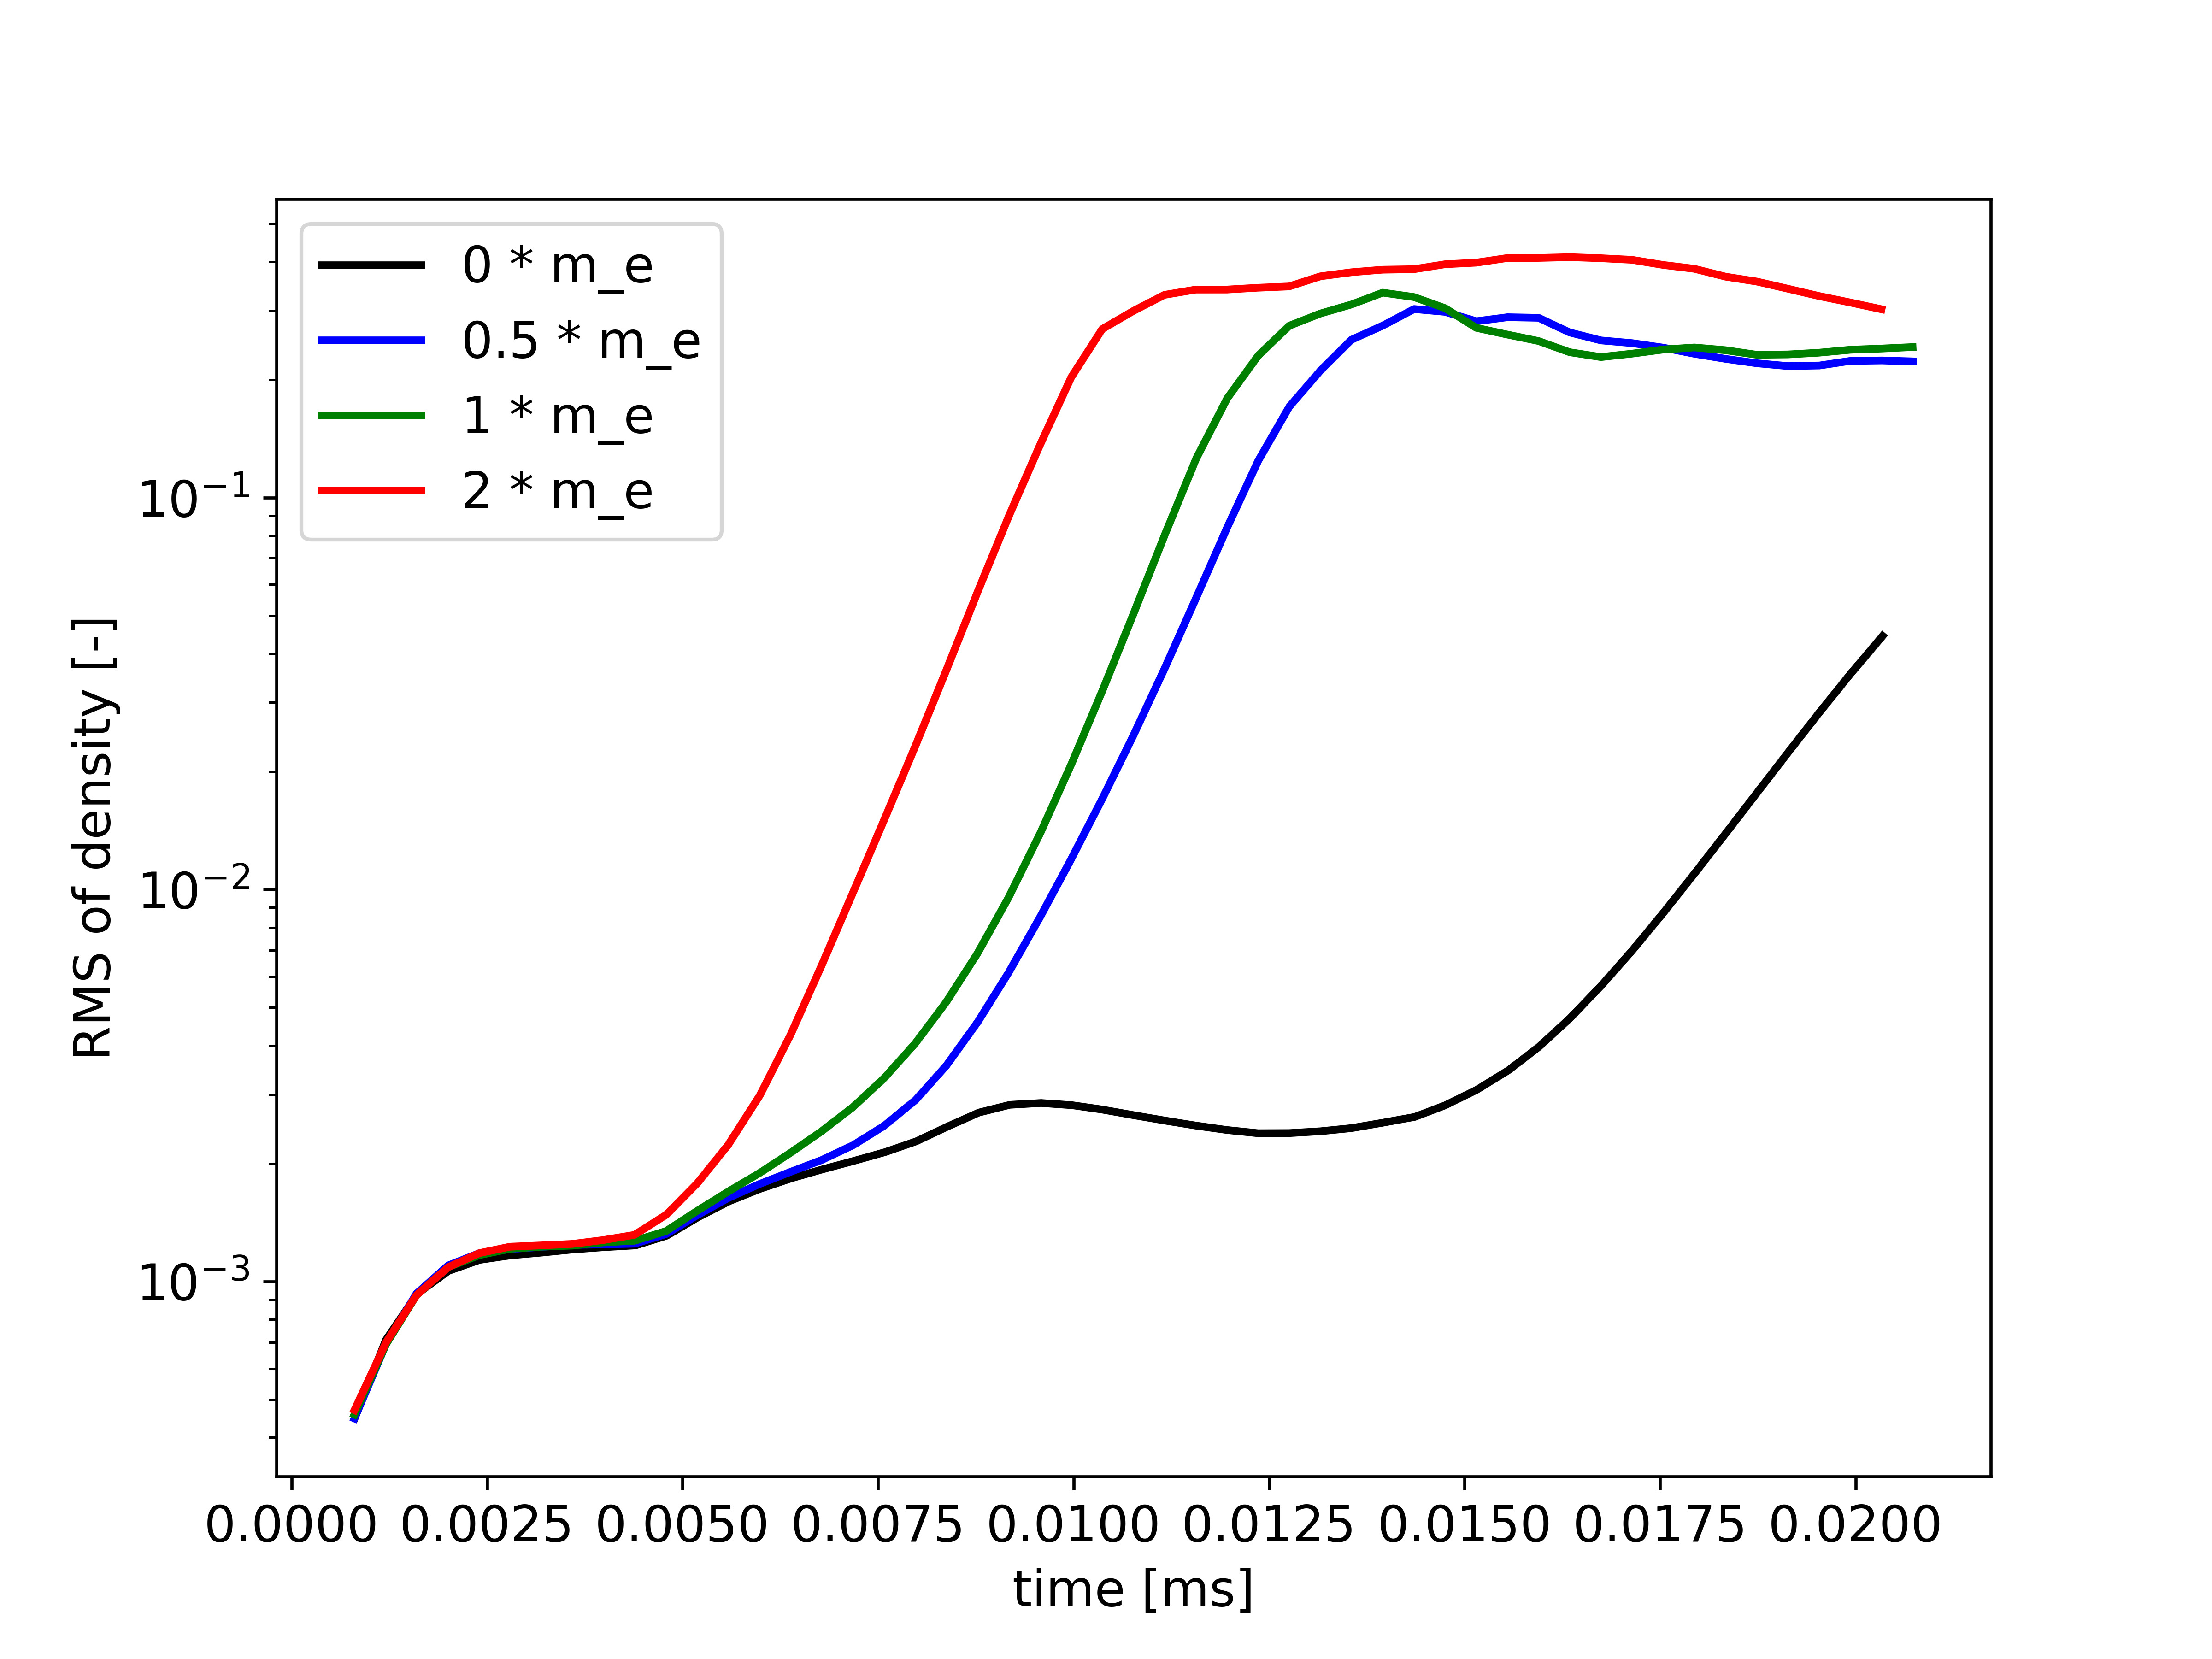
\includegraphics[width=1\textwidth]{schemes/RMSn_meScan.jpg}
		\subcaption{RMS of density $n_i$}
	\end{subfigure}
	\begin{subfigure}[t]{0.45\textwidth}
		\centering
		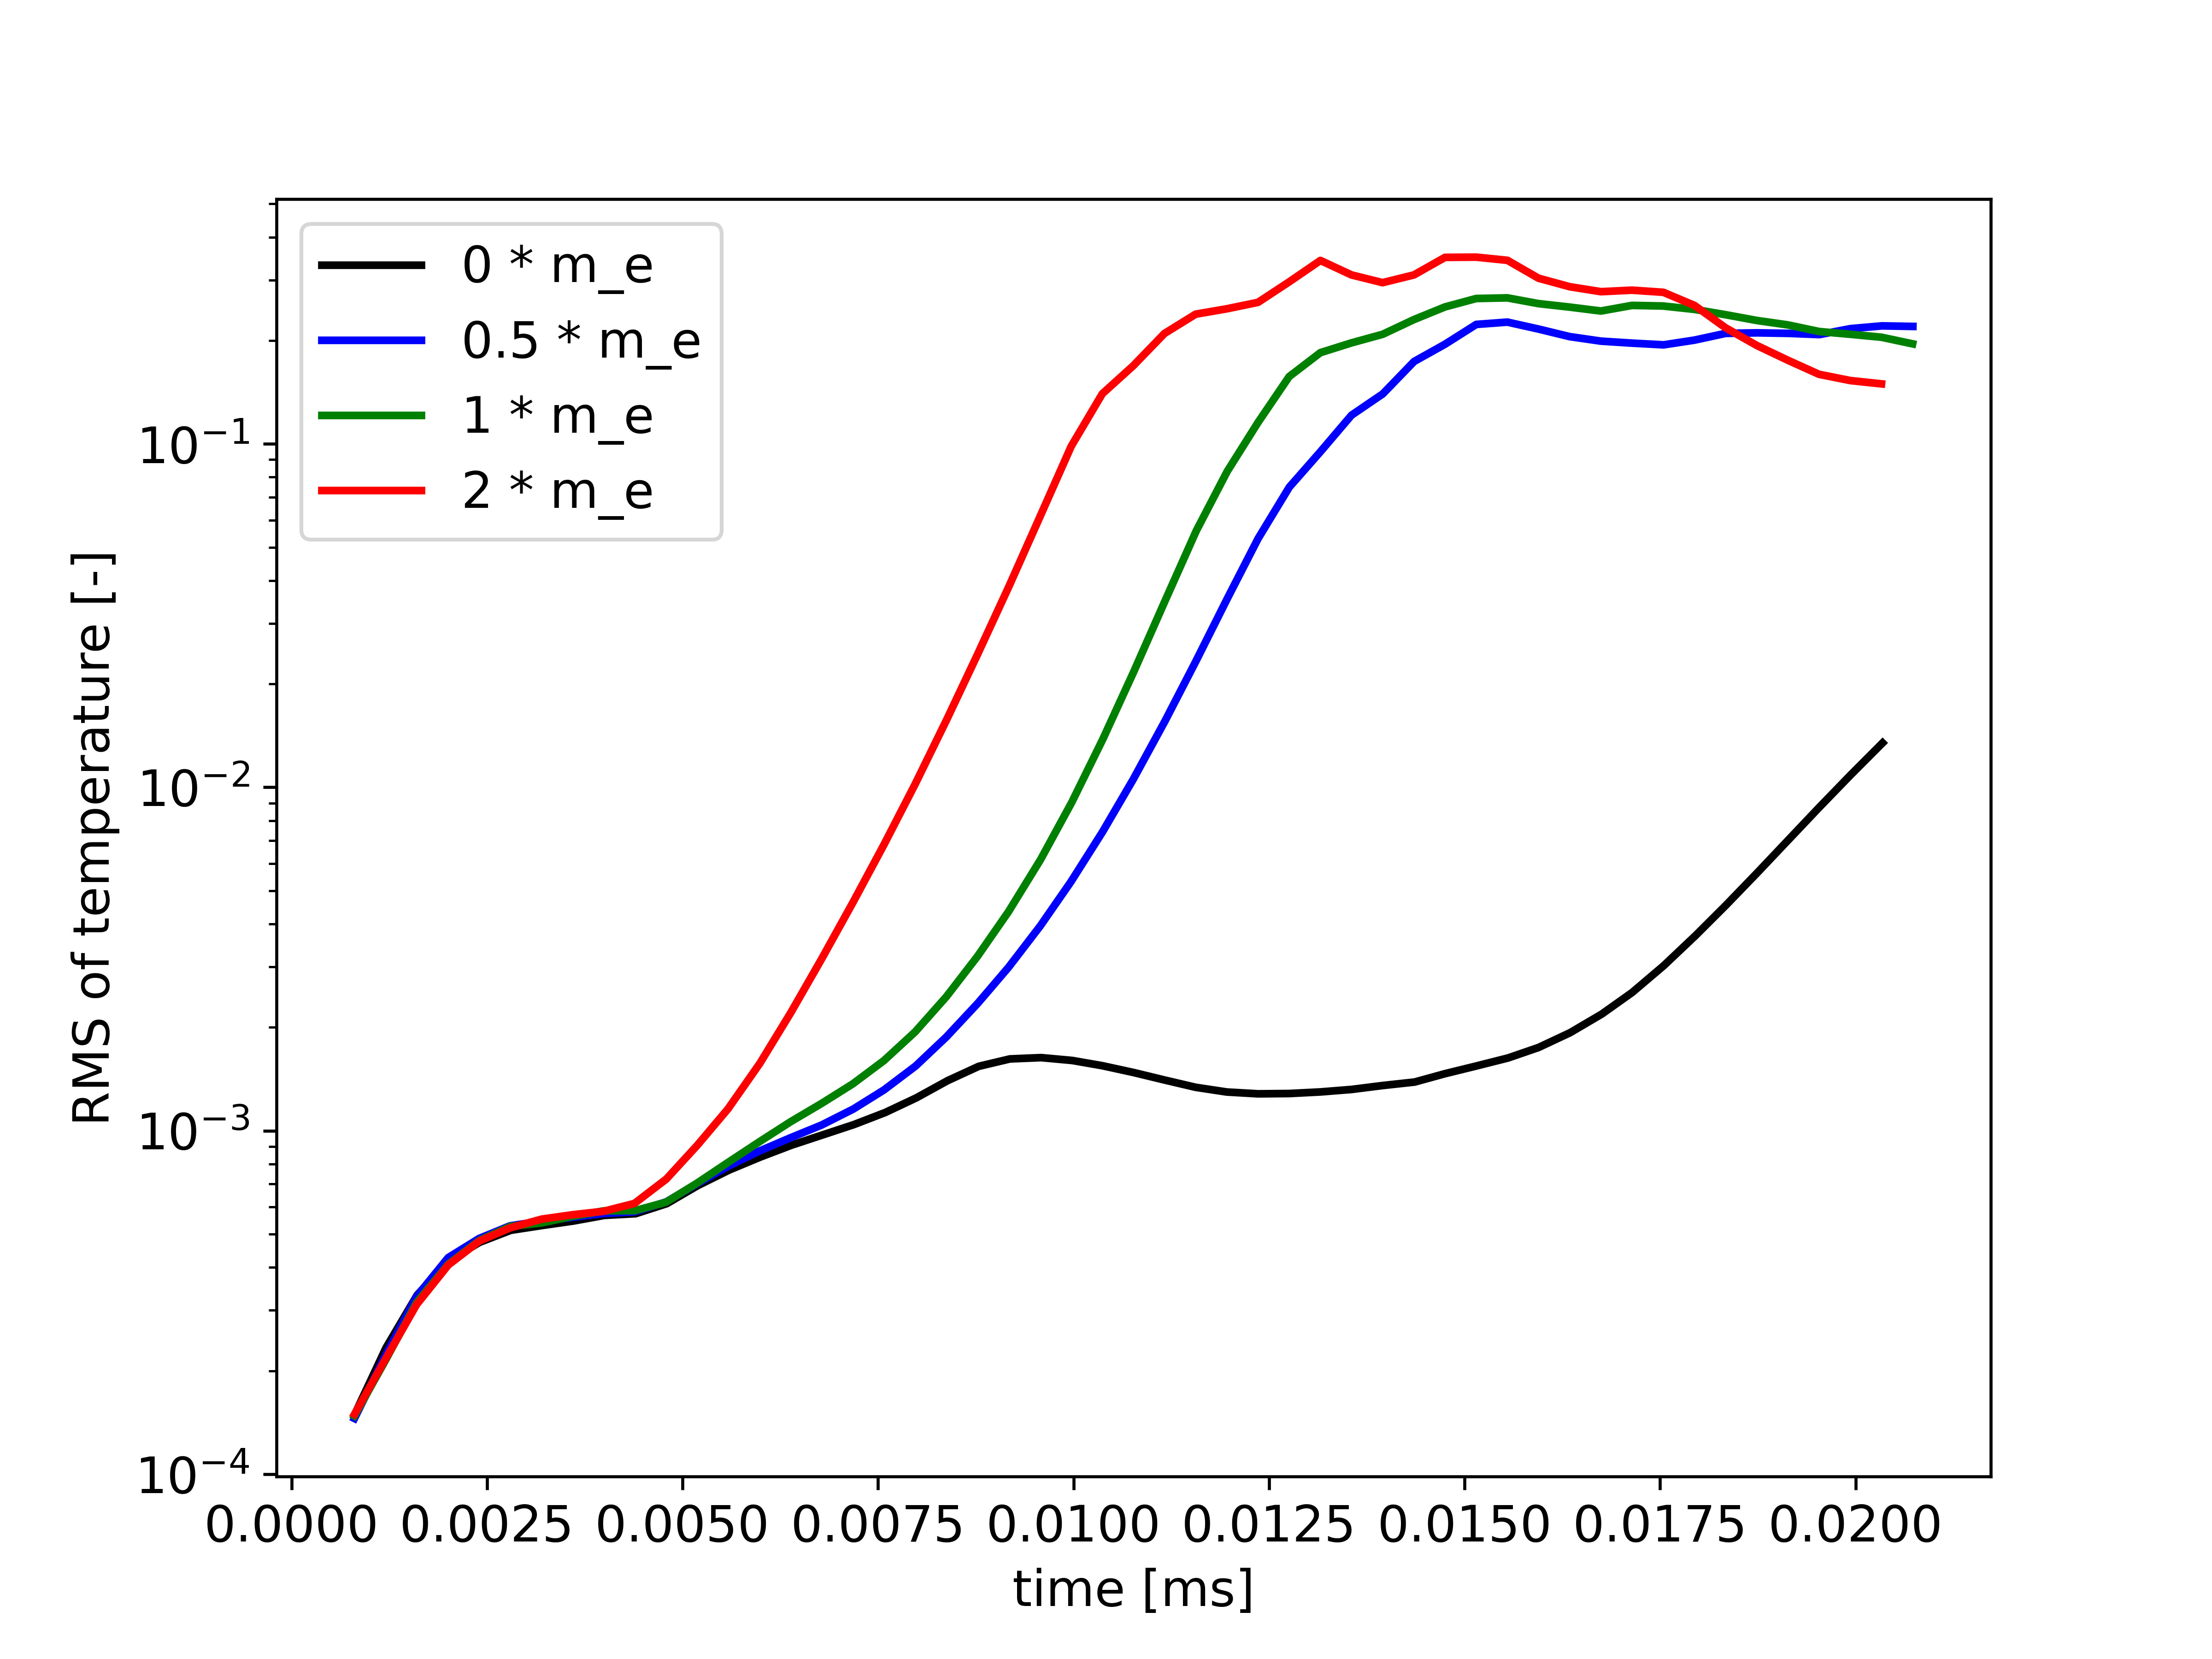
\includegraphics[width=1\textwidth]{schemes/RMST_meScan.jpg}
		\subcaption{RMS of temperature $T_i$}
	\end{subfigure}
	\caption{Evolution of the the root mean square deviation for different values of $m_e$. The electron mass is artificially increased and the 0 factor corresponds effectively to the electrostatic reference}
	\label{fig:CIRC_meScan}
\end{figure}


\subsubsection{Magnetic induction}

Second, we modify the value of the reference $\beta_0$ that appears in the dimensionless equations for the term $\partial_t A_\parallel$ in the parallel electric field. From a physical standpoint, we actually change the vacuum permeability $\mu_0$ as the reference pressure $n_0T_0$ and magnetic field strength $B_0$ remain unchanged for the rest of the model. All simulations are run with the true value of the electron mass, so the base case $0\beta_0$ is equivalent to the green line in the $m_e$ scan above. In Fig. \ref{fig:CIRC_betaScan}, we observe that perturbations grow faster the stronger $\beta_0$ is. For the case $1\beta_0$, we also included flutter as a dashed line, and we see there that the growth rate is reduced again to levels below the electron inertial case. 

\begin{figure}[H]\centering
	\begin{subfigure}[t]{0.45\textwidth}
		\centering
		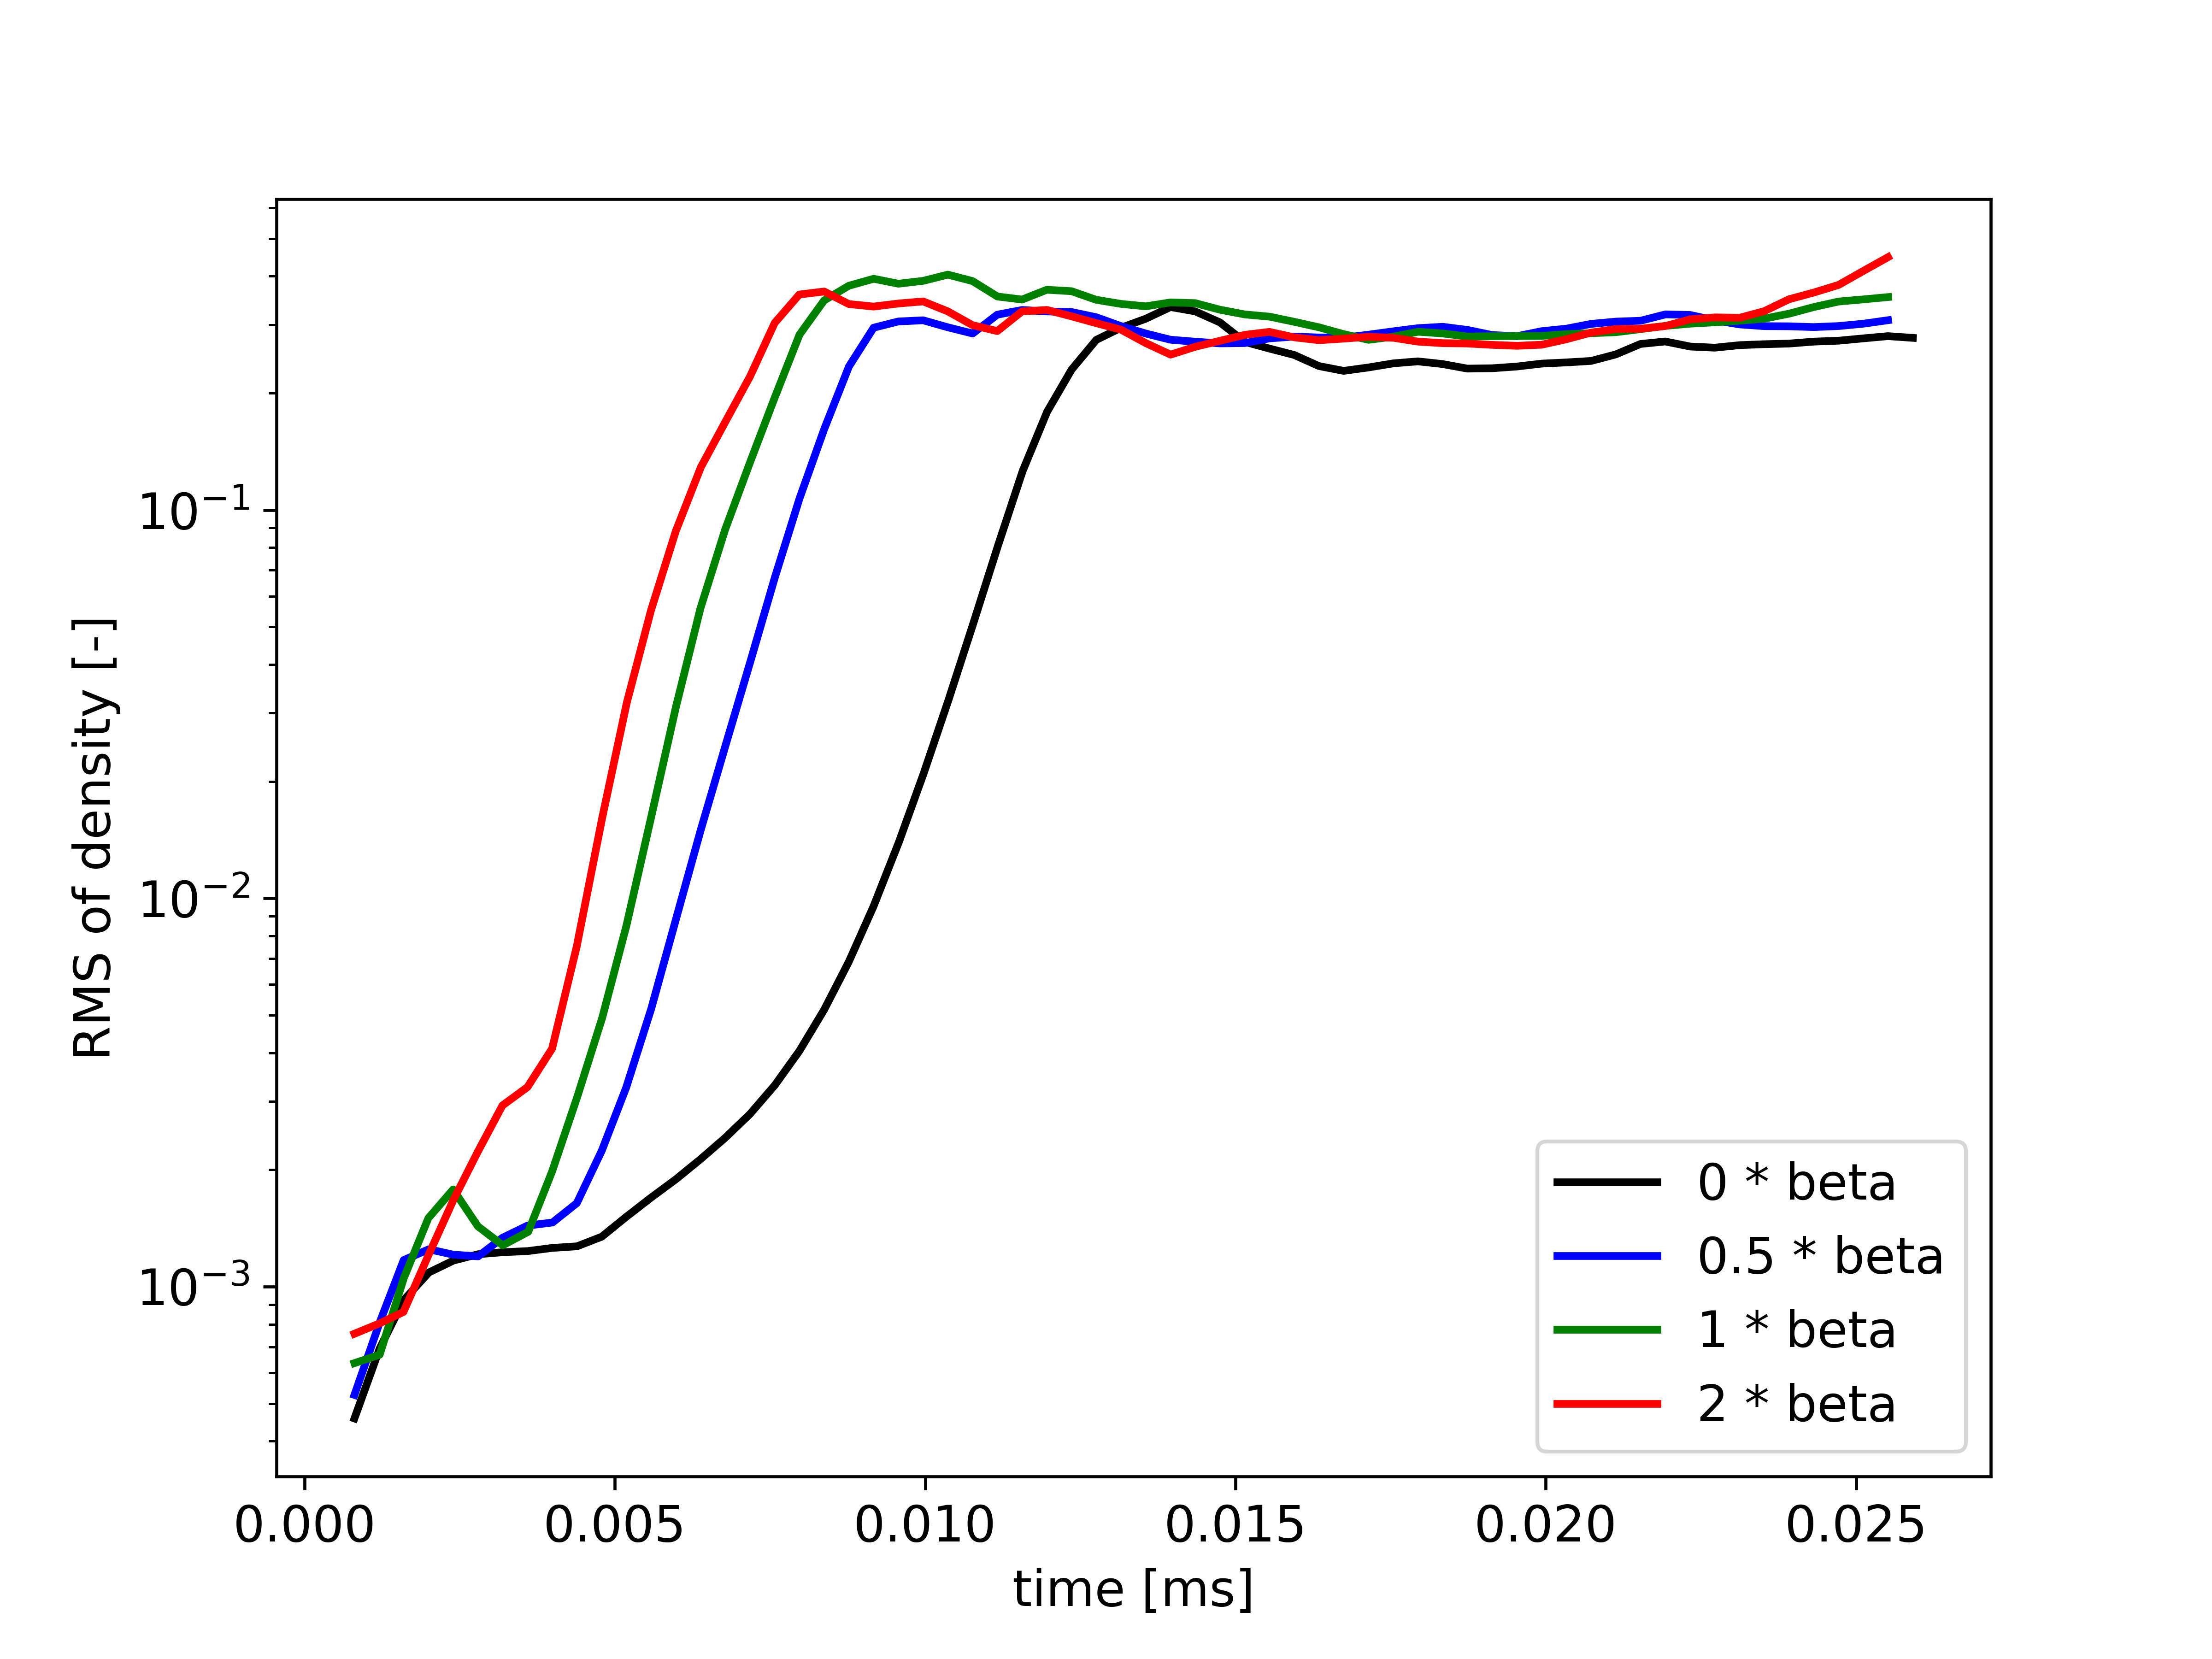
\includegraphics[width=1\textwidth]{schemes/RMSn_betaScan.jpg}
		\subcaption{RMS of density $n_i$}
	\end{subfigure}
	\begin{subfigure}[t]{0.45\textwidth}
		\centering
		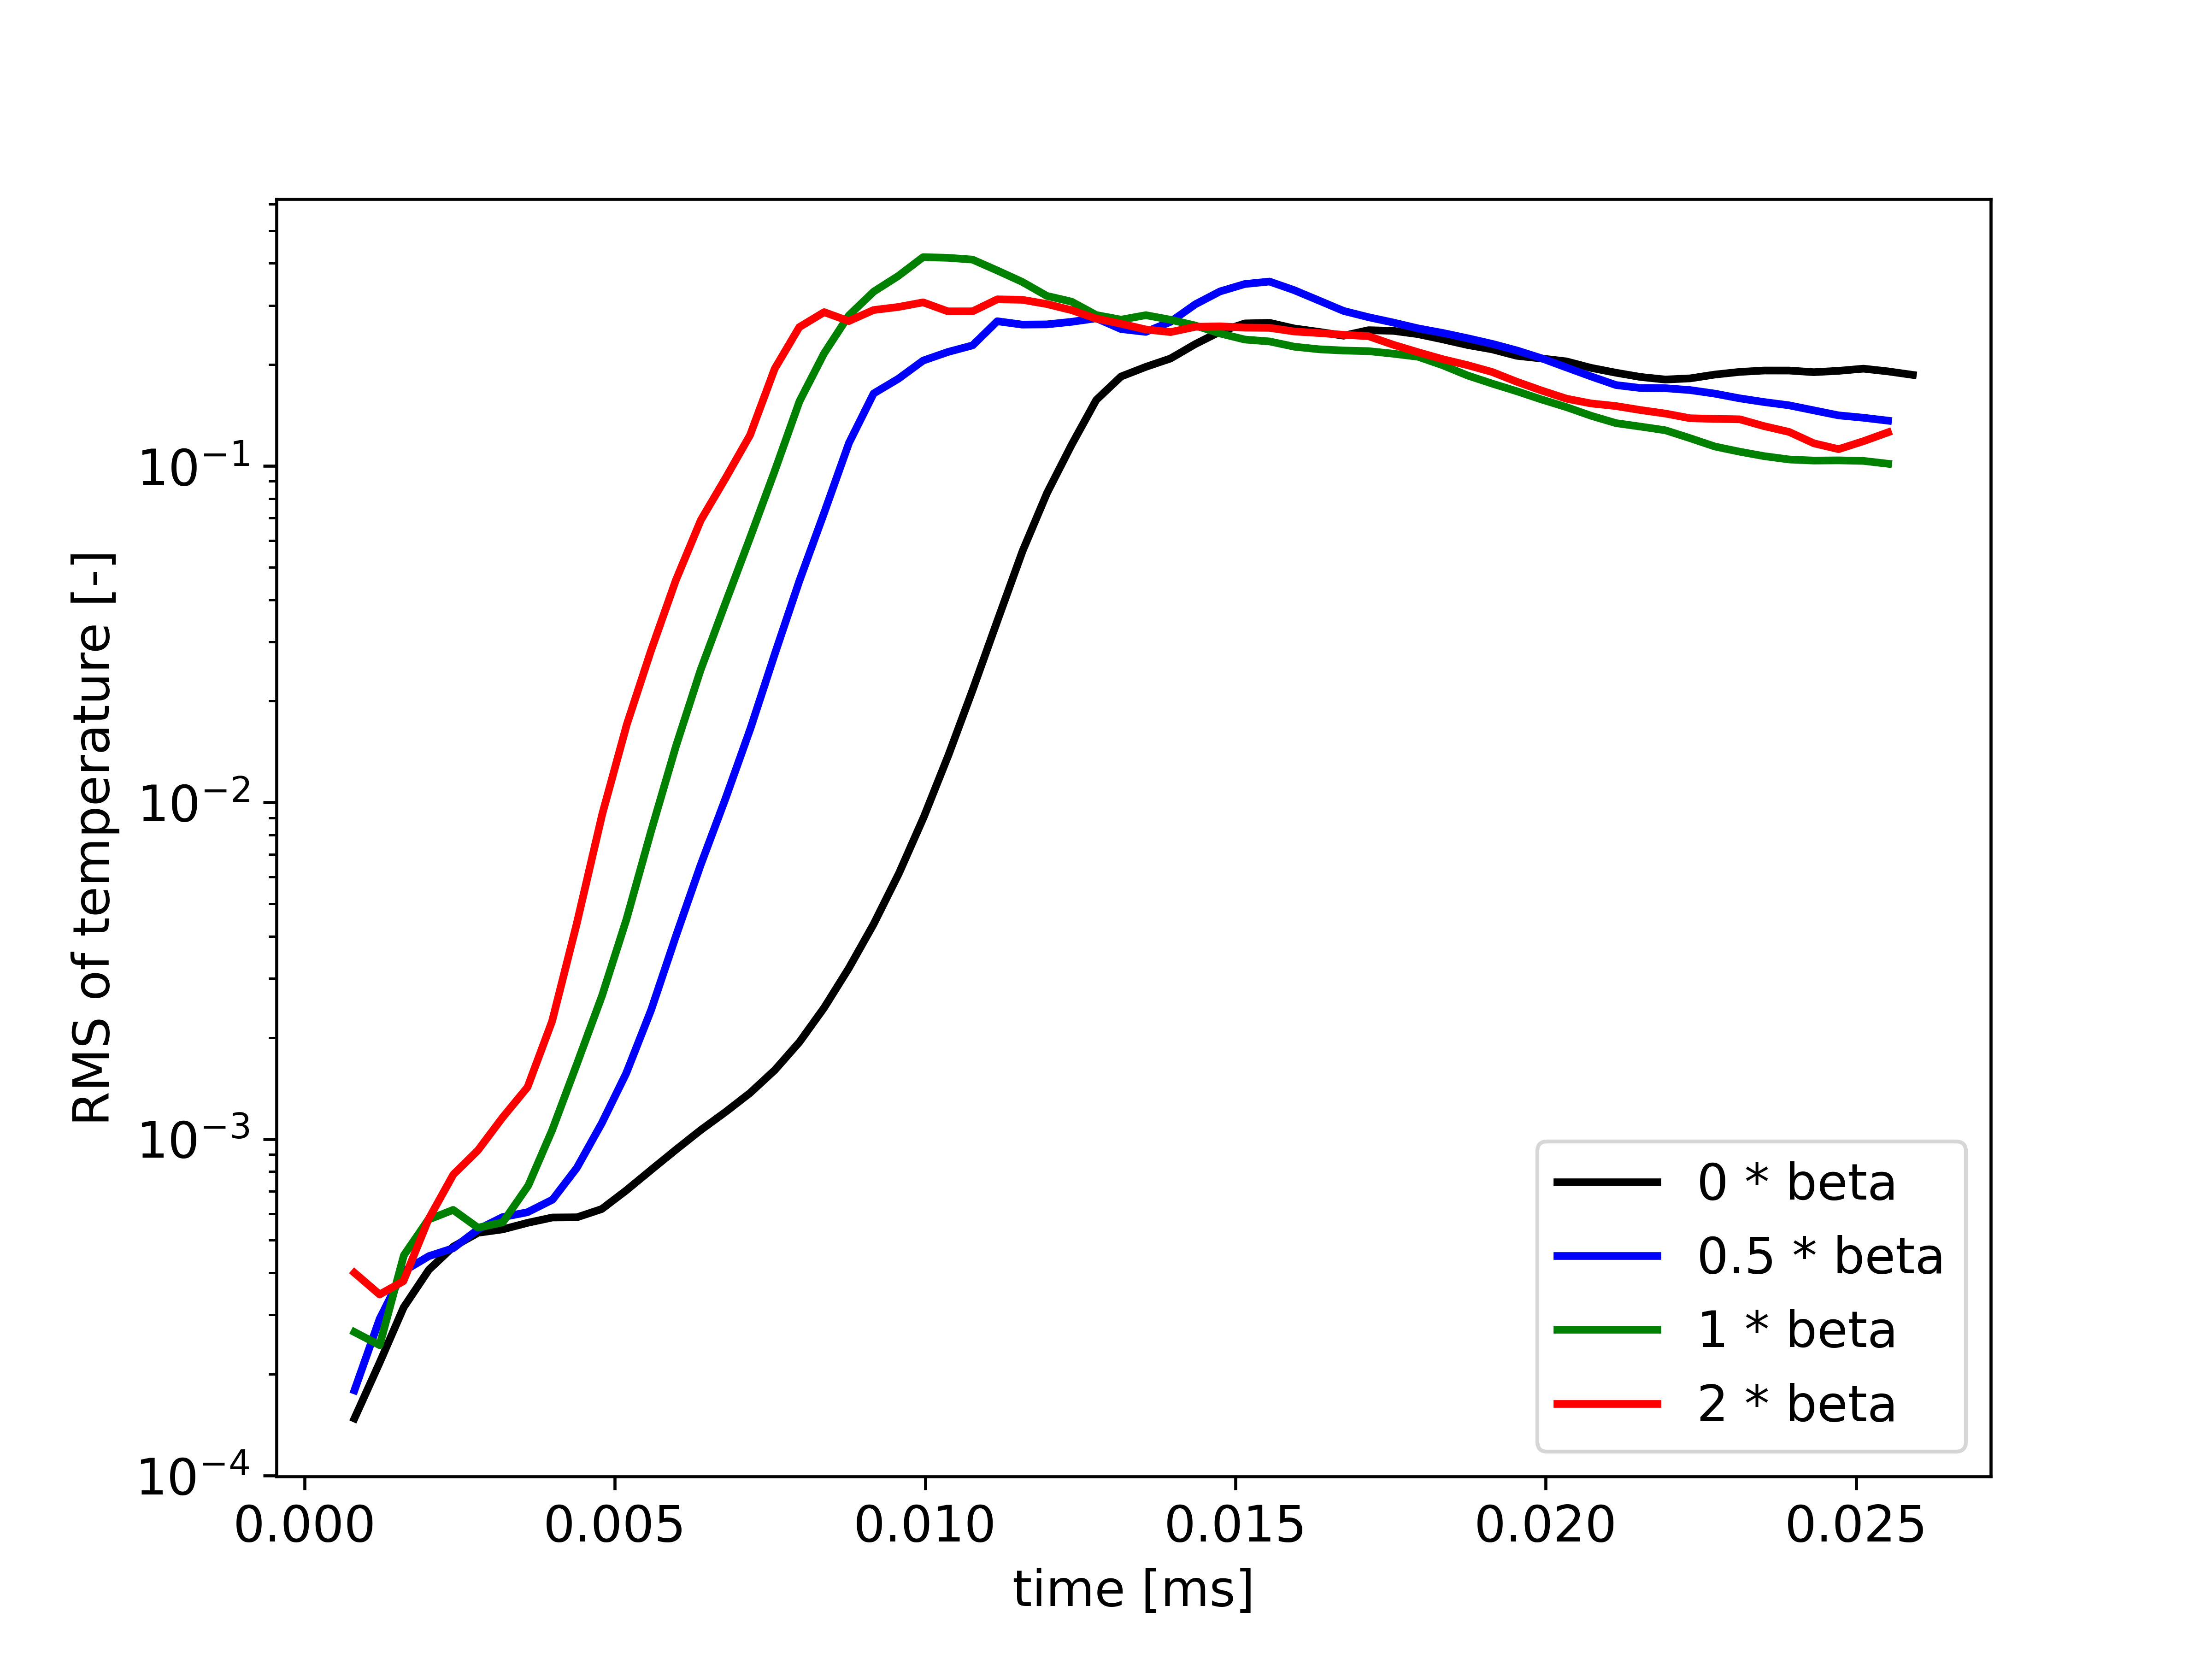
\includegraphics[width=1\textwidth]{schemes/RMST_betaScan.jpg}
		\subcaption{RMS of temperature $T_i$}
	\end{subfigure}
	\caption{Evolution of the the root mean square deviation for different values of $\beta$. The  is artificially increased and the 0 factor corresponds effectively to the electrostatic with electron inerita. The electron mass for all scenarios is physical (factor 1 in Fig. \ref{fig:CIRC_meScan}).}
	\label{fig:CIRC_betaScan}
\end{figure}

For both the $m_e$ and $\beta_0$ scan, we could see that the linear growth corresponds to the expectations from the linear analysis. As the effects of electron inertia and magnetic induction get stronger, plasma perturbations grow faster and reach their saturation point faster. Note that the saturation levels are similar for all scenarios, so the used RMS metric is not very adapted to analyze the subsequent nonlinear phase of the simulation. \\

The results here can however not be correlated one-to-one to the dispersion relation. In the SOLEDGE3X model, interchange instabilities also contribute to the rise of perturbation, and the simulation was run with the energy conservation equation and hence ion and electron temperature gradients add an additional source of instability. The dispersion relation was calculated without curvature effects and using an isothermal assumption, but the general expected trend is still observed. 







